%Version 3.1 December 2024
% See section 11 of the User Manual for version history
%%%%%%%%%%%%%%%%%%%%%%%%%%%%%%%%%%%%%%%%%%%%%%%%%%%%%%%%%%%%%%%%%%%%%%
% https://www.editorialmanager.com/isfi/default2.aspx
% https://www.springernature.com/gp/authors/campaigns/latex-author-support
% https://link.springer.com/journal/10796/submission-guidelines
%
%%%%%%%%%%%%%%%%%%%%%%%%%%%%%%%%%%%%%%%%%%%%%%%%%%%%%%%%%%%%%%%%%%%%%%%
% Information Systems Frontiers (Springer, SCIE, Q2)
% -왜 적합한가: 정책, 법, 책임 있는 AI, 데이터 거버넌스 등 정보시스템과 사회적 규제의 접점을 다룸.
% -SCIE 여부: JCR/SCIE 등재.
% -APC: 하이브리드 → OA 선택 안 하면 APC 없음.
% -장점: 사회적·정책적 맥락과 기술 결합 논문을 환영.
% -“빠른 accept + 게재비 0원 + SCIE”를 만족하고, **당신의 논문 주제(LLM 기반 규제 모니터링·AI % Governance Informatics)**와 가장 잘 맞는 곳은:
%   1) Government Information Quarterly (Elsevier, Q1)
%   2) Information Systems Frontiers (Springer, Q2)
%   3) 보조 후보: IEEE Intelligent Systems (IEEE, SCIE)

%%\documentclass[referee,sn-basic]{sn-jnl}% referee option is meant for double line spacing
\documentclass[pdflatex,sn-mathphys-num]{sn-jnl}% Math and Physical Sciences Numbered Reference Style

%%%% Standard Packages
%%<additional latex packages if required can be included here>

\usepackage{graphicx}%
\usepackage{multirow}%
\usepackage{amsmath,amssymb,amsfonts}%
\usepackage{amsthm}%
\usepackage{mathrsfs}%
\usepackage[title]{appendix}%
\usepackage{xcolor}%
\usepackage{textcomp}%
\usepackage{manyfoot}%
\usepackage{booktabs}%
\usepackage{algorithm}%
\usepackage{algorithmicx}%
\usepackage{algpseudocode}%
\usepackage{listings}%
%%%%

%% ------------- Geunsik Area : Start ----------------------

\usepackage{natbib} % author–year 권장

% How to separate languages (e.g., ko, en) for paper writing
\usepackage{ifthen} % 조건문 사용
\newcommand{\lang}{en} % Language: ko 또는 en 으로 설정
\newcommand{\anonymous}{false} % Author: true 또는 false으로 설정

% How to support Korean language with the 'latexmkrc' file in www.overleaf.com
\usepackage{kotex}

% How to print date, hour, and minute to maintain the current version of the paper.
% Append the below statement in the 'abstract' section.
% For example, write "[Notice] This document was compiled on: \today\ at \currenttime." 
\usepackage[short,nodayofweek,level,24hr]{datetime}

% 날짜/시간 포맷 정의
\newdateformat{customdate}{\shortmonthname[\THEMONTH]-\twodigit{\THEDAY}-\THEYEAR \ \currenttime}

% for pseudo code
\usepackage{algorithm}
%\usepackage[noend]{algpseudocode}

% for using a number symbol (\ding{3})
\usepackage{pifont}

% Text highlight and color (e.g. \hl, \textcolor )
\usepackage{xcolor,color,soul}
%\usepackage{soul}

% Hyperlinks to content
%\usepackage[linktocpage=true]{hyperref}
\usepackage{hyperref}
%\usepackage[hidelinks]{hyperref}


% The color styles for hyperlinks
%   urlcolor     = blue, %Colour for external hyperlinks

\hypersetup{
  colorlinks   = false, %Colours links instead of ugly boxes
  urlcolor     = blue, %Colour for external hyperlinks
  linkcolor    = black,  %Colour of internal links
  citecolor    = black  %Colour of citations, could be ``red''
}

% How to support a code listing
%\usepackage{listings}

% set the default code style
\lstset{
    frame=tb, % draw a frame at the top and bottom of the code block
    tabsize=4, % tab space width
    showstringspaces=false, % don't mark spaces in strings
    numbers=left, % display line numbers on the left
    commentstyle=\color{green}, % comment color
    keywordstyle=\color{blue}, % keyword color
    stringstyle=\color{red} % string color
}

% to use toprule in table
%\usepackage{booktabs}
\usepackage{multirow}

% page number
\pagestyle{plain}

%% ------------- Geunsik Area : End --------------------------

%%%%%=============================================================================%%%%
%%%%  Remarks: This template is provided to aid authors with the preparation
%%%%  of original research articles intended for submission to journals published 
%%%%  by Springer Nature. The guidance has been prepared in partnership with 
%%%%  production teams to conform to Springer Nature technical requirements. 
%%%%  Editorial and presentation requirements differ among journal portfolios and 
%%%%  research disciplines. You may find sections in this template are irrelevant 
%%%%  to your work and are empowered to omit any such section if allowed by the 
%%%%  journal you intend to submit to. The submission guidelines and policies 
%%%%  of the journal take precedence. A detailed User Manual is available in the 
%%%%  template package for technical guidance.
%%%%%=============================================================================%%%%

%% as per the requirement new theorem styles can be included as shown below
\theoremstyle{thmstyleone}%
\newtheorem{theorem}{Theorem}%  meant for continuous numbers
%%\newtheorem{theorem}{Theorem}[section]% meant for sectionwise numbers
%% optional argument [theorem] produces theorem numbering sequence instead of independent numbers for Proposition
\newtheorem{proposition}[theorem]{Proposition}% 
%%\newtheorem{proposition}{Proposition}% to get separate numbers for theorem and proposition etc.

\theoremstyle{thmstyletwo}%
\newtheorem{example}{Example}%
\newtheorem{remark}{Remark}%

\theoremstyle{thmstylethree}%
\newtheorem{definition}{Definition}%

\raggedbottom
%%\unnumbered% uncomment this for unnumbered level heads


\begin{document}

% Article: Title 

%\title{(DRAFT) FALCON: Leveraging LLMs for Efficient AI Regulatory Monitoring and Insight Extraction}

%\title{LexSense: LLM-Driven Regulatory Monitoring for Scalable AI Governance}
% 라틴어 Lex (법)와 Sense (탐지)를 결합 → 논문 주제(규제 감지, 법적 감시)를 직관적으로 드러냄.

%\title{AI Governance Informatics: The LexSense Framework for LLM-Driven Regulatory Monitoring and Compliance}

\title{LexSense: Multilingual AI for Inclusive Access to Legal and Government Information}

% Article: Author
\ifthenelse{\equal{\anonymous}{false}}{%
%%=============================================================%%
%% GivenName	-> \fnm{Joergen W.}
%% Particle	-> \spfx{van der} -> surname prefix
%% FamilyName	-> \sur{Ploeg}
%% Suffix	-> \sfx{IV}
%% \author*[1,2]{\fnm{Joergen W.} \spfx{van der} \sur{Ploeg} 
%%  \sfx{IV}}\email{iauthor@gmail.com}
%%=============================================================%%

\author*[1]{\fnm{Geunsik} \sur{Lim}}\email{leemgs@g.skku.edu}

\affil*[1]{\orgdiv{The Department of Electrical and Computer Engineering}, \orgname{Sungkyunkwan University}, \orgaddress{\street{2066, Seobu-ro, Jangan-gu}, \city{Suwon}, \postcode{2066}, \state{Gyeonggi-do}, \country{South Korea}}}


}{ %else

\author*[1]{\fnm{Anonymous } \sur{Author(s)}\email{xxx@xxx.edu}

\affil*[1]{\orgdiv{Department}, \orgname{Organization Name}, \orgaddress{\street{Street}, \city{City}, \postcode{xxxxxx}, \state{State}, \country{Country}}}

        $^{\textsuperscript{}}$\
        {\color{blue} \\ (DRAFT), Printed on \customdate\today \ for IJCAI 2026 }
        }
} % end of if


% Article: Abstract
\ifthenelse{\equal{\lang}{ko}}{%
\begin{abstract}
생성형 AI의 급격한 성장은 거버넌스와 컴플라이언스에 대한 수요를 강화하였다. 
기존의 모니터링 도구—수작업 보고서, 키워드 알림, 정적 추적기—는 
전 세계적으로 빠르게 변화하는 규제를 따라잡지 못한다. 
본 연구에서는 (1) 실시간 변화 탐지, (2) 의미론적 데이터 수집, 
(3) LLM 기반 보고를 통합한 \textbf{LexSense}라는 통합 프레임워크를 제안한다. 
새로운 분류 체계를 통해 다양한 관할권과 언어에서 규제 문서, 계약서, 소송, 
AI 자산 공개를 정밀하게 분류할 수 있다. 
EU, 미국, 한국 데이터셋을 대상으로 한 실험에서 91\%의 정확도, 
분석가 업무량 82\% 감소, 보고 속도 70\% 향상이라는 결과를 달성하였다. 
다국어 테스트와 소거(ablation) 실험을 통해 강건성이 확인되었다. 
또한 전체 코드, 데이터셋, Docker 기반 파이프라인을 공개하여 재현성을 보장한다. 
기술적 성과를 넘어, LexSense는 공정성 인식 튜닝, 편향 감사, 
프라이버시 보호형 모니터링을 통합하였다. 
이러한 기여는 \textbf{AI 거버넌스 정보학(AI Governance Informatics)}이라는 
새로운 연구 방향을 정립하며, 확장 가능하고 투명하며 책임 있는 
AI 거버넌스를 위한 배포 가능한 컴플라이언스 인프라와 개념적 토대를 함께 제공한다.
\end{abstract}



%\textbf{Keywords:}: 생성형 인공지능, AI 거버넌스 및 컴플라이언스, 대규모 언어 모델(LLM), 자동화 규제 모니터링, 책임 있는 AI 시스템


}{%
% -------------------- English Version --------------------
\abstract{The rapid growth of generative AI has intensified demands for governance and compliance. Existing monitoring tools---manual reports, keyword alerts, and static trackers---cannot keep pace with dynamic, global regulatory changes. We introduce \textbf{LexSense}, a unified framework combining (1) real-time change detection, (2) semantic data acquisition, and (3) LLM-driven reporting. A novel taxonomy enables fine-grained classification of governance documents, contracts, lawsuits, and AI asset releases across jurisdictions and languages. Experiments on EU, U.S., and Korean datasets achieve 91\% accuracy, 82\% less analyst effort, and 70\% faster reporting than manual baselines. Cross-lingual tests and ablations confirm robustness. We release full code, datasets, and Dockerized pipelines for reproducibility. Beyond technical gains, LexSense integrates fairness-aware tuning, bias audits, and privacy-preserving monitoring. Together, these contributions establish \textbf{AI Governance Informatics} as a new research direction, offering both a deployable compliance infrastructure and a conceptual foundation for scalable, transparent, and responsible AI governance. 
}


\keywords{AI Governance Informatics, Large Language Models (LLMs), Regulatory Monitoring, Compliance Automation, Cross-lingual Information Systems}
}


%%\pacs[JEL Classification]{D8, H51}
%%\pacs[MSC Classification]{35A01, 65L10, 65L12, 65L20, 65L70}

\maketitle

% Article: Introduction
\section{Introduction}\label{sec:introduction}
\ifthenelse{\equal{\lang}{ko}}{%
 법률, 규제, 정부 정보는 시민의 권리와 의무, 공공 서비스 이용, 사회·경제적 참여의 근간을 이룬다. 그러나 이러한 정보는 복잡한 전문 용어, 파편화된 출처, 그리고 언어 장벽으로 인해 비전문가와 다국어 공동체에게 여전히 접근하기 어려운 자원으로 남아 있다 \cite{zhong2020legalai, chalkidis2020legalbert}. 이민자, 소상공인, 취약 계층, 그리고 자국어가 공식 문서의 언어와 다른 사람들에게 이러한 장벽은 정보 격차를 심화시키고 공정한 공공 서비스 접근을 저해한다 \cite{aletras2016echr}.

여러 관할권에서 법령, 판례, 계약, 행정 공지는 서로 다른 언어와 형식으로 지속적으로 갱신된다. 유럽연합의 AI 법안 \cite{EUAIAct2024}과 같은 대규모 규제 프레임워크는 다국어로 공표되지만, 일반 시민이 이를 자신의 언어로 정확히 이해하고 자신의 상황에 적용하기는 쉽지 않다. 기존의 접근 방식—키워드 검색, 수작업 번역, 정적 정보 포털—은 의미적 깊이가 부족하거나, 최신성을 유지하지 못하거나, 저자원 언어를 충분히 다루지 못한다 \cite{niklaus2023multilegal}.

본 논문에서는 다양한 관할권과 언어에 걸쳐 거버넌스 관련 정보를 \textbf{수집·분류·분석·요약}하도록 설계된 다국어 AI 프레임워크인 \textbf{LexSense}를 제안한다. LexSense는 (1) 자동 변화 탐지, (2) 다국어 자연어 처리 \cite{conneau2020xlmr, xue2021mt5}, (3) 개념 드리프트(concept drift) 모니터링 \cite{gama2014drift}, (4) 근거 기반(evidence-grounded) 분석 \cite{lewis2020rag}, (5) 대규모 언어 모델(LLM) 기반 보고 \cite{openai2023gpt4, touvron2023llama2}를 하나의 엔드투엔드 파이프라인으로 통합한다. 핵심 목표는 규제 준수를 대신하는 것이 아니라, 법률 및 정부 지식에 대한 \emph{포용적 접근}을 지원하는 것이다.
~\\
본 연구의 기여는 세 가지다.
\textbf{첫째, 다국어 접근성 프레임워크:} 변화 탐지, 다국어 분류, 근거 기반 요약, LLM 보고를 결합한 모듈형 프레임워크를 설계·구현하여, 비전문가와 다국어 사용자가 공공 정보에 접근하는 데 따르는 언어적·기술적 장벽을 낮춘다 \cite{devlin2019bert, reimers2020multilingual}.
\textbf{둘째, 다국어 벤치마크(GovSense-1k):} 근거 주석이 포함된 1,200건의 거버넌스·계약·소송·자산 관련 레코드로 구성된 다국어 벤치마크를 공개하고, 이를 영어·한국어·프랑스어에 걸쳐 검증하였다 \cite{chalkidis2022lexglue, hendrycks2021cuad}.
\textbf{셋째, 포괄적 평가:} 영어·한국어·프랑스어에 대한 주 평가와 스페인어·아랍어·베트남어에 대한 스트레스 테스트를 수행하여, 다국어·근거 기반 AI가 공공 정보 접근성을 향상시킬 수 있음을 정량적으로 입증하였다 \cite{nllb2022, hu2020xtreme}.

이러한 기술적 기여를 넘어, 본 연구는 책임 있는 배포를 위한 사실성(factuality), 투명성, 인간 감독(human oversight) 요구사항을 함께 논의한다 \cite{ji2023hallucination, maynez2020faithfulness, weidinger2021taxonomy}. 종합하면, LexSense는 자연어 처리, 법·정책 정보학, 책임 있는 AI의 교차점에서, 공공 지식에 대한 \textbf{포용적 접근}을 위한 실용적이면서도 확장 가능한 인프라를 제시한다 \cite{bommasani2021foundation}.



}{%
% -------------------- English Version --------------------
Legal, regulatory, and government information underpins citizens' rights and obligations, access to public services, and socioeconomic participation. Yet such information remains difficult to access for non-experts and multilingual communities because of complex terminology, fragmented sources, and language barriers \cite{zhong2020legalai, chalkidis2020legalbert}. For immigrants, small business owners, vulnerable populations, and people whose native language differs from that of official documents, these barriers widen information gaps and hinder equitable access to public services \cite{aletras2016echr}.

Across jurisdictions, statutes, case law, contracts, and administrative notices are continuously updated in different languages and formats. Large regulatory frameworks such as the European Union AI Act \cite{EUAIAct2024} are published in multiple languages, yet ordinary citizens still struggle to understand them accurately in their own language and to apply them to their own circumstances. Existing approaches---keyword search, manual translation, and static information portals---lack semantic depth, fail to stay current, or provide insufficient coverage of low-resource languages \cite{niklaus2023multilegal}.

In this paper, we introduce \textbf{LexSense}, a multilingual AI framework designed to \textbf{collect, classify, analyze, and summarize} governance-related information across different jurisdictions and languages. LexSense integrates (1) automated change detection, (2) multilingual natural language processing \cite{conneau2020xlmr, xue2021mt5}, (3) concept-drift monitoring \cite{gama2014drift}, (4) evidence-grounded analysis \cite{lewis2020rag}, and (5) large language model (LLM)-based reporting \cite{openai2023gpt4, touvron2023llama2} into a single end-to-end pipeline. Its central goal is not to replace regulatory compliance functions but to support \emph{inclusive access} to legal and governmental knowledge.
~\\
Our contributions are threefold.
\textbf{First, a multilingual accessibility framework:} we design and implement a modular framework that combines change detection, multilingual classification, evidence-grounded summarization, and LLM reporting, lowering the linguistic and technical barriers that non-experts and multilingual users face when accessing public information \cite{devlin2019bert, reimers2020multilingual}.
\textbf{Second, a multilingual benchmark (GovSense-1k):} we release a multilingual benchmark of 1,200 governance, contract, lawsuit, and asset-related records with evidence annotations, validated across English, Korean, and French \cite{chalkidis2022lexglue, hendrycks2021cuad}.
\textbf{Third, comprehensive evaluation:} we conduct a main evaluation on English, Korean, and French, together with stress tests on Spanish, Arabic, and Vietnamese, quantitatively demonstrating that multilingual, evidence-grounded AI can improve access to public information \cite{nllb2022, hu2020xtreme}.

Beyond these technical contributions, we discuss factuality, transparency, and human oversight requirements for responsible deployment \cite{ji2023hallucination, maynez2020faithfulness, weidinger2021taxonomy}. Taken together, LexSense offers a practical yet scalable infrastructure for \textbf{inclusive access} to public knowledge, at the intersection of natural language processing, legal and policy informatics, and responsible AI \cite{bommasani2021foundation}.

}


% Article: Background
\section{Background}\label{sec:background}
\ifthenelse{\equal{\lang}{ko}}{%
본 장에서는 법률·정부 정보 접근을 위한 기존 접근 방식을 검토하고, 그 한계를 강조하며, 다국어 NLP/LLM의 발전을 정리하고, \textbf{포용적 접근(inclusive access)}을 위한 다국어 AI 프레임워크의 필요성을 명확히 한다.

\subsection{공공 법률·정부 정보 접근 방식}
공공 법률 및 정부 정보에 대한 접근은 오랫동안 정보 격차의 원천이었다. \textbf{키워드 기반 검색과 정적 포털} (예: 정부 웹사이트, RSS)은 배포가 쉽지만 표면적 일치에 의존하여 불필요한 잡음을 발생시키거나 미묘한 의미를 놓치기 쉽다 \cite{zhong2020legalai}. \textbf{수작업 번역 및 상담}은 정확한 맥락을 제공하지만 느리고 비용이 많이 들며 확장성이 부족하다 \cite{aletras2016echr}. \textbf{정보 검색 데이터베이스} (예: 법령·판례 검색 시스템)는 방대한 자료를 통합하지만 다국어 지원이 제한적이고, 비전문가가 이해하기 어려운 형식으로 결과를 제공한다 \cite{niklaus2023multilegal}.

\begin{table}[h]
\centering
\small
\begin{tabular}{p{0.25\linewidth}p{0.65\linewidth}}
\toprule
접근 방식 & 한계 \\
\midrule
키워드 검색 & 맥락 부족, 높은 오탐률 \\
수작업 번역·상담 & 정확하나 비용 높고 느림 \\
정보 검색 DB & 제한된 다국어 지원, 비전문가 이해 어려움 \\
\bottomrule
\end{tabular}
\caption{기존 공공 정보 접근 방식의 한계.}
\end{table}

\subsection{법률·정책 텍스트를 위한 다국어 NLP와 LLM}
초기 연구들은 규칙 기반 조항 추출, 계약 분석, 법률 검색에 NLP를 적용하였다 \cite{chalkidis2020legalbert}. Transformer 기반 다국어 인코더(mBERT, XLM-R, mT5)의 등장은 언어 간 전이(cross-lingual transfer)를 통해 저자원 언어에서도 강건한 표현 학습을 가능케 하였다 \cite{devlin2019bert, conneau2020xlmr, xue2021mt5}. 최근 GPT-4, LLaMA-2와 같은 대규모 언어 모델(LLMs)은 강력한 의미 추론과 요약, 그리고 다국어 이해 능력을 보여준다 \cite{openai2023gpt4, touvron2023llama2}. 그러나 이러한 능력을 \emph{시민 대면(citizen-facing) 정보 접근}에 통합한 프레임워크는 여전히 드물다. LexGLUE, LegalBench, CUAD와 같은 벤치마크는 법률 NLP 과제를 표준화하였으나 \cite{chalkidis2022lexglue, guha2023legalbench, hendrycks2021cuad}, 대부분 영어 중심이며 다국어 포용성을 충분히 다루지 않는다.

\subsection{근거 기반 생성과 책임 있는 AI}
병행 연구에서는 사실성(factuality)과 투명성을 강조한다. 검색 증강 생성(RAG)은 외부 근거에 기반하여 생성의 신뢰성을 높이며 \cite{lewis2020rag}, 요약의 충실성(faithfulness)과 환각(hallucination) 탐지에 관한 연구는 LLM 출력의 사실 검증 필요성을 부각한다 \cite{maynez2020faithfulness, ji2023hallucination}. 동시에 Model Cards, 언어 모델의 사회적 위험 분류 등은 배포 시 해석 가능성과 윤리의 중요성을 강조한다 \cite{mitchell2021modelcards, bender2021stochastic, weidinger2021taxonomy}. 그러나 대부분은 시민 대면 접근성 시스템에 내재화되지 않았다.

\subsection{연구 공백}
현행 방법들은 관할권과 언어를 넘나드는 확장 가능하고, 최신성이 유지되며, 근거에 기반한 시민 대면 정보 접근을 제공하지 못한다. 더 나아가 사실성·투명성·인간 감독과 같은 안전장치는 시스템 설계에 거의 통합되지 않았다 \cite{gama2014drift}. 이는 본 연구의 동기를 제공한다: 법률 및 정부 지식에 대한 \textbf{포용적 접근}을 지원하는 다국어·근거 기반 LLM 프레임워크.

\begin{table}[t]
\centering
\small
\resizebox{\columnwidth}{!}{%
\begin{tabular}{p{2.2cm} p{3.3cm} p{5.0cm}}
\toprule
 & \textbf{법률 정보 검색} & \textbf{다국어 포용적 접근 (본 연구)} \\
\midrule
주요 초점 & 검색, 조항/요소 추출, 법률 QA & \textbf{변화 탐지} $\rightarrow$ \textbf{다국어 분류} $\rightarrow$ \textbf{근거 기반 요약·LLM 보고} (엔드투엔드) \\
시간성 & 정적/주기적 업데이트 & \textbf{준실시간} 변화 감지 및 드리프트 대응 \\
언어 & 주로 단일 언어(영어 중심) & \textbf{다국어} (영·한·불 + 저자원 스트레스 테스트) \\
대상 사용자 & 법률 전문가 & \textbf{비전문가·다국어 공동체} \\
핵심 방법 & 규칙/IR + 전통적 NLP & \textbf{LLM 추론}, 근거 기반 설명 가능성 \\
출력 & 문서/조각 & \textbf{출처 포함 구조화·근거 연결 요약} \\
\bottomrule
\end{tabular}
}
\caption{법률 정보 검색과 \emph{다국어 포용적 접근}의 개념적 차이.}
\label{tab:conceptual}
\end{table}


}{%
This section reviews existing approaches to accessing legal and government information, highlights their limitations, situates advances in multilingual NLP/LLMs, and clarifies the need for a multilingual AI framework for \textbf{inclusive access}.

\subsection{Approaches to Public Legal and Government Information}
Access to public legal and government information has long been a source of information inequality. \textbf{Keyword-based search and static portals} (e.g., government websites, RSS) are easy to deploy but rely on surface-level matches, often generating irrelevant noise or missing nuanced meaning \cite{zhong2020legalai}. \textbf{Manual translation and advisory services} provide accurate context but are slow, costly, and lack scalability \cite{aletras2016echr}. \textbf{Information-retrieval databases} (e.g., statute and case-law search systems) consolidate large corpora but offer limited multilingual support and return results in formats that non-experts find difficult to understand \cite{niklaus2023multilegal}.

\begin{table}[h]
\centering
\small
\begin{tabular}{p{0.25\linewidth}p{0.65\linewidth}}
\toprule
Approach & Limitation \\
\midrule
Keyword search & Misses context, high false positives \\
Manual translation/advice & Accurate but costly and slow \\
IR databases & Limited multilingual support, hard for non-experts \\
\bottomrule
\end{tabular}
\caption{Limitations of existing public-information access approaches.}
\end{table}

\subsection{Multilingual NLP and LLMs for Legal and Policy Texts}
Early work applied NLP to rule-based clause extraction, contract analysis, and legal retrieval \cite{chalkidis2020legalbert}. The emergence of transformer-based multilingual encoders (mBERT, XLM-R, mT5) enabled robust representation learning even for low-resource languages via cross-lingual transfer \cite{devlin2019bert, conneau2020xlmr, xue2021mt5}. Recent large language models (LLMs) such as GPT-4 and LLaMA-2 demonstrate strong semantic reasoning, summarization, and multilingual understanding \cite{openai2023gpt4, touvron2023llama2}. However, frameworks that integrate these capabilities into \emph{citizen-facing} information access remain scarce. Benchmarks such as LexGLUE, LegalBench, and CUAD have standardized legal NLP tasks \cite{chalkidis2022lexglue, guha2023legalbench, hendrycks2021cuad}, but most are English-centric and do not sufficiently address multilingual inclusiveness.

\subsection{Evidence-Grounded Generation and Responsible AI}
Parallel research emphasizes factuality and transparency. Retrieval-augmented generation (RAG) grounds generation in external evidence to improve reliability \cite{lewis2020rag}, while work on summarization faithfulness and hallucination detection highlights the need to fact-check LLM outputs \cite{maynez2020faithfulness, ji2023hallucination}. At the same time, Model Cards and taxonomies of social risks from language models stress the importance of interpretability and ethics in deployment \cite{mitchell2021modelcards, bender2021stochastic, weidinger2021taxonomy}. Yet most remain external to citizen-facing accessibility systems.

\subsection{Research Gap}
Current methods fail to deliver scalable, current, and evidence-grounded citizen-facing information access across jurisdictions and languages. Moreover, safeguards such as factuality, transparency, and human oversight are rarely integrated into system design \cite{gama2014drift}. This motivates our work: a multilingual, evidence-grounded LLM framework that supports \textbf{inclusive access} to legal and governmental knowledge.

\begin{table}[t]
\centering
\small
\resizebox{\columnwidth}{!}{%
\begin{tabular}{p{2.2cm} p{3.3cm} p{5.0cm}}
\toprule
 & \textbf{Legal Information Retrieval} & \textbf{Multilingual Inclusive Access (This Work)} \\
\midrule
Primary Focus & Retrieval, clause/element extraction, legal QA & \textbf{Change detection} $\rightarrow$ \textbf{multilingual classification} $\rightarrow$ \textbf{evidence-grounded summarization / LLM reporting} (end-to-end) \\
Temporality & Static/periodic updates & \textbf{Near real-time} change detection and drift-aware adaptation \\
Languages & Mostly monolingual (English-centric) & \textbf{Multilingual} (EN/KO/FR + low-resource stress tests) \\
Target Users & Legal experts & \textbf{Non-experts and multilingual communities} \\
Method Core & Rules/IR + classical NLP & \textbf{LLM reasoning}, evidence-linked explainability \\
Outputs & Documents/fragments & \textbf{Structured, evidence-linked summaries} with provenance \\
\bottomrule
\end{tabular}
}
\caption{Conceptual distinction between Legal Information Retrieval and \emph{Multilingual Inclusive Access}.}
\label{tab:conceptual}
\end{table}


}



% Article: Design 
\section{LexSense: Design and Implementation}\label{sec:lexsense}
\ifthenelse{\equal{\lang}{ko}}{%
\begin{figure}[t]
  \centering
  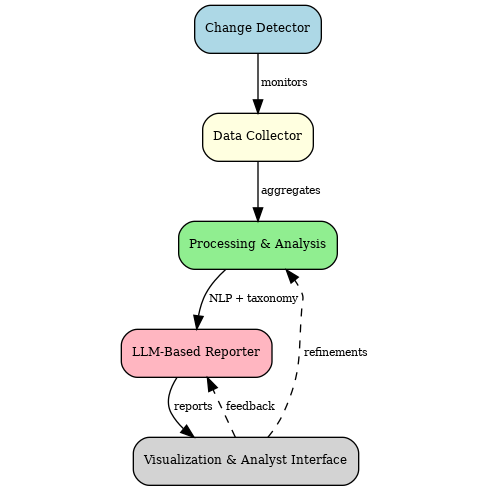
\includegraphics[width=0.9\linewidth]{fig-system_architecture.png}
  \caption{\textbf{LexSense 시스템 아키텍처.} 다섯 개의 모듈형 구성요소—탐지, 수집, 분석, 보고, 시각화—가 함께 작동하여 확장 가능하고, 다국어이며, 근거에 기반한 법률·정부 정보 접근을 가능하게 한다.}
  \label{fig:architecture}
\end{figure}

설계 목표는 세 가지이다: (1) \textbf{다국어 포용성(multilingual inclusiveness)} — 다양한 언어의 시민이 자신의 언어로 공공 정보에 접근할 수 있도록 함 \cite{conneau2020xlmr, xue2021mt5}; (2) \textbf{근거 기반 신뢰성(evidence-grounded reliability)} — 요약과 답변을 원문 근거에 연결하여 사실성을 보장함 \cite{lewis2020rag, maynez2020faithfulness}; (3) \textbf{투명성(transparency)} — 비전문가가 이해하고 검증할 수 있는 구조화된 설명 가능한 출력을 생성함 \cite{mitchell2021modelcards}.

\subsection{시스템 아키텍처}
그림~\ref{fig:architecture}은 시스템 아키텍처를 보여주며, 이는 다섯 개의 핵심 구성 요소로 이루어져 있다.
~\\
\textbf{1) 변화 탐지기(Change Detector):} 정부 포털, 법령·판례 데이터베이스, 공공 공지, 뉴스 매체를 지속적으로 모니터링하여 새로운 콘텐츠나 업데이트를 감지한다. 분산 크롤러와 스트리밍 파이프라인을 활용해 거의 실시간으로 후속 분석을 촉발한다 \cite{gama2014drift, niklaus2023multilegal}.
~\\
\textbf{2) 데이터 수집기(Data Collector):} 정책 데이터베이스, 법률 문서, 행정 공지 등 이질적 정보를 집계한다. API 기반 수집과 적응형 웹 스크래핑 모듈을 병행하여 다양한 관할권과 언어를 포괄한다 \cite{nllb2022}.
~\\
\textbf{3) 처리 및 분석 모듈(Processing and Analysis Module):} 개체 인식, 조항 추출, 이벤트 분류를 위해 다국어 NLP 파이프라인을 적용한다. Transformer 기반 다국어 인코더(mBERT, XLM-R)를 도메인 특화 분류체계와 결합하여 언어 간 전이를 통한 구조화된 표현을 가능케 한다 \cite{devlin2019bert, conneau2020xlmr}.
~\\
\textbf{4) LLM 기반 리포터(LLM-Based Reporter):} GPT-4, LLaMA-2 및 법률 도메인 특화 모델을 활용하여 구조화된 요약을 생성하고, 핵심 조항을 강조하며, 다중 출처 정보를 종합한다 \cite{openai2023gpt4, touvron2023llama2}. 또한 근거 구간에 기반한 검색 증강 생성(RAG)과 인간 피드백 루프를 적용하여 사실 정확성을 높이고 환각을 줄인다 \cite{lewis2020rag, ji2023hallucination}.
~\\
\textbf{5) 시각화 및 사용자 인터페이스(Visualization and User Interface):} 대시보드와 인터랙티브 요약을 제공하며, 평이한 언어(plain language) 설명과 근거 링크를 함께 표시한다. 비전문가의 이해와 신뢰를 돕도록 설계 원칙을 반영하였다 \cite{mitchell2021modelcards, ouyang2022instructgpt}.

\subsection{구현 세부사항}
시스템은 마이크로서비스 지향 아키텍처로 구현되어 모듈성과 확장성을 극대화한다. \textbf{데이터 수집:} 분산 크롤러가 Apache Kafka 큐에서 실행되어 50개 이상의 소스로부터 병렬적이고 내결함성 있는 데이터 수집을 수행한다 \cite{niklaus2023multilegal}. \textbf{전처리 파이프라인:} 다국어 인코더를 법률·정책 코퍼스에 파인튜닝하여 조항 추출 성능을 향상시키고 불필요한 잡음을 줄인다 \cite{devlin2019bert, conneau2020xlmr}. \textbf{의미 검색:} 문장 임베딩 기반 검색을 통해 다국어 근거 구간을 정렬한다 \cite{reimers2019sbert, reimers2020multilingual}. \textbf{피드백 루프:} 사용자 및 전문가 교정 내용은 기록 후 재학습에 반영되어 분류 정확도와 요약 품질을 점진적으로 향상시킨다. \textbf{재현성:} 전체 구현, 데이터 준비 스크립트, Docker 기반 환경을 GitHub에 공개하여 재현성을 보장한다 \cite{mitchell2021modelcards}.

\subsection{설계 원칙}
세 가지 설계 원칙이 아키텍처를 형성하였다: \textbf{(1) 모듈성(Modularity)} — 각 하위 시스템(탐지, 수집, 분석, 보고, 시각화)이 독립적으로 업데이트될 수 있어 새로운 LLM이나 다국어 데이터 소스와의 통합이 용이하다 \cite{devlin2019bert, conneau2020xlmr}; \textbf{(2) 효율성(Efficiency)} — 엔드투엔드 자동화를 통해 탐지와 요약 간의 지연을 최소화하여 준실시간 정보 접근을 가능케 한다 \cite{reimers2019sbert, lewis2020rag}; \textbf{(3) 투명성(Transparency)} — 산출물이 구조화되고 설명 가능하며 근거에 연결되도록 설계되어, 비전문가의 신뢰와 검증 가능성을 뒷받침한다 \cite{mitchell2021modelcards, maynez2020faithfulness}. 전체적으로, 본 설계는 확장성뿐 아니라 재현성, 사용성, 책임 있는 배포를 강조하며, 자동화된 정보 접근이 과학적으로 엄밀하면서도 다국어 공동체에 실질적으로 포용적일 수 있도록 한다 \cite{weidinger2021taxonomy, bommasani2021foundation}.

}{%


\begin{figure}[t]
  \centering
  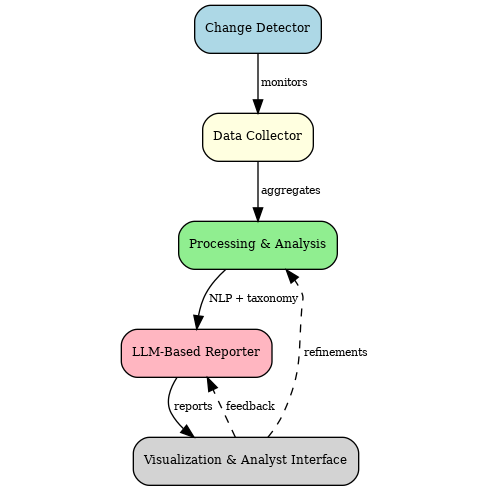
\includegraphics[width=0.9\linewidth]{fig-system_architecture}
  \caption{\textbf{LexSense System Architecture.} Five modular components—detection, collection, analysis, reporting, and visualization—work together to enable scalable, multilingual, and evidence-grounded access to legal and government information.}
  \label{fig:architecture}
\end{figure}


The design goals are threefold: (1) \textbf{multilingual inclusiveness}, so that citizens speaking diverse languages can access public information in their own language \cite{conneau2020xlmr, xue2021mt5}; (2) \textbf{evidence-grounded reliability}, linking summaries and answers to source evidence to ensure factuality \cite{lewis2020rag, maynez2020faithfulness}; and (3) \textbf{transparency}, generating structured, explainable outputs that non-experts can understand and verify \cite{mitchell2021modelcards}.


\subsection{System Architecture}
Figure~\ref{fig:architecture} illustrates the system's architecture, which is composed of five core components:
~\\
\textbf{1) Change Detector:} Continuously monitors government portals, statute and case-law databases, public notices, and news outlets for new or updated content. Using distributed crawlers and streaming pipelines, it triggers downstream analysis in near real time \cite{gama2014drift, niklaus2023multilegal}.
~\\
\textbf{2) Data Collector:} Aggregates heterogeneous information from policy databases, legal filings, and administrative notices. Both API-based ingestion and adaptive web-scraping modules are employed to ensure coverage across jurisdictions and languages \cite{nllb2022}.
~\\
\textbf{3) Processing and Analysis Module:} Applies multilingual NLP pipelines for entity recognition, clause extraction, and event classification. Transformer-based multilingual encoders (mBERT, XLM-R) are integrated with domain-specific taxonomies, enabling structured representation through cross-lingual transfer \cite{devlin2019bert, conneau2020xlmr}.
~\\
\textbf{4) LLM-Based Reporter:} Employs large language models (GPT-4, LLaMA-2, and legal-domain models) to generate structured summaries, highlight key clauses, and synthesize multi-source information \cite{openai2023gpt4, touvron2023llama2}. Retrieval-augmented generation (RAG) grounded in evidence spans, together with a human feedback loop, improves factual accuracy and reduces hallucinations \cite{lewis2020rag, ji2023hallucination}.
~\\
\textbf{5) Visualization and User Interface:} Provides dashboards and interactive summaries that present plain-language explanations alongside evidence links. Guided by design principles for trust and interpretability, the interface helps non-experts understand and trust the output \cite{mitchell2021modelcards, ouyang2022instructgpt}.

\subsection{Implementation Details}
The system is implemented using a microservice-oriented architecture to maximize modularity and scalability. \textbf{Data Ingestion:} distributed crawlers run on Apache Kafka queues, enabling parallel and fault-tolerant data collection from over 50 sources \cite{niklaus2023multilegal}. \textbf{Preprocessing Pipelines:} multilingual encoders are fine-tuned on legal and policy corpora to improve clause extraction and reduce noise \cite{devlin2019bert, conneau2020xlmr}. \textbf{Semantic Retrieval:} sentence-embedding-based retrieval aligns multilingual evidence spans \cite{reimers2019sbert, reimers2020multilingual}. \textbf{Feedback Loop:} user and expert corrections are logged and reintegrated into retraining, gradually refining classification accuracy and summary quality over time. \textbf{Reproducibility:} we release the full implementation, dataset preparation scripts, and Dockerized environments on GitHub \cite{mitchell2021modelcards}.



\subsection{Design Principles}
Three guiding principles shaped our architecture: \textbf{(1) Modularity}, where each subsystem—detection, collection, analysis, reporting, and visualization—can be independently updated, facilitating integration with emerging LLMs or multilingual data sources \cite{devlin2019bert, conneau2020xlmr}; \textbf{(2) Efficiency}, where end-to-end automation minimizes latency between detection and summarization, enabling near real-time information access \cite{reimers2019sbert, lewis2020rag}; and \textbf{(3) Transparency}, where outputs are structured, explainable, and evidence-linked, supporting trust and verifiability for non-experts \cite{mitchell2021modelcards, maynez2020faithfulness}. Overall, the design emphasizes not only scalability but also reproducibility, usability, and responsible deployment, ensuring that automated information access is both scientifically rigorous and practically inclusive for multilingual communities \cite{weidinger2021taxonomy, bommasani2021foundation}.


}



% Article: Evaluation
\section{Evaluation}\label{sec:evaluation}
\ifthenelse{\equal{\lang}{ko}}{%
우리는 다국어 정보 접근 프레임워크인 \textbf{LexSense}를 분류 정확도, 지연(latency), 효율성, 사용자 만족도 등 여러 차원에서 평가하였다. 본 평가의 목표는 다양한 언어의 대규모 법률·정부 정보를 처리하고, 이해하기 쉬운 인사이트를 생성하며, 비전문가와 다국어 사용자의 정보 접근을 지원하는 데 있어 시스템의 효과성을 입증하는 것이다 \cite{zhong2020legalai, niklaus2023multilegal}.

\subsection{데이터셋}
평가에는 3개월 동안 수집된 1,200건의 규제 및 법적 업데이트가 포함된 데이터셋을 사용하였다. 여기에는 정책 발표, 법적 제출 문서, 여러 관할권의 행정 가이드라인이 포함된다. 추가로, 기술 자산의 분류 및 맥락화 능력을 평가하기 위해 250건의 AI 모델 및 데이터셋 공개 자료를 통합하였다. 정량적 평가를 보완하기 위해, 법률 지원 실무자와 다국어 공동체 구성원을 포함한 12명의 참여자를 대상으로 사용자 연구도 수행하였다 \cite{EUAIAct2024, chalkidis2022lexglue}.

\subsection{평가지표}
성능 평가는 네 가지 주요 지표를 통해 수행되었다: (1) 정밀도(Precision)와 재현율(Recall) — NLP와 정보 검색에서 널리 사용됨 \cite{devlin2019bert, raffel2020t5}; (2) 지연(Latency) — 변화 탐지부터 구조화된 요약 생성까지 걸린 시간으로 정의됨 \cite{reimers2019sbert, lewis2020rag}; (3) 사용자 만족도(User Satisfaction) — 1~5 점 척도로 사용자 신뢰 및 요약의 유용성을 반영 \cite{mitchell2021modelcards, ouyang2022instructgpt}; (4) 워크플로우 효율성(Workflow Efficiency) — 수작업 대비 준비 시간 감소율로 측정 \cite{maynez2020faithfulness, gama2014drift}.

\subsection{정량적 결과}
표~\ref{tab:performance}는 네 가지 주요 범주별 성능을 요약한다. 시스템은 일관되게 높은 정밀도와 재현율을 달성하면서 낮은 지연 시간을 유지하였다. 벤치마크는 GPT-3, GPT-4, LLaMA-2와 같은 최신 LLM 평가 결과와 비교하였다 \cite{brown2020gpt3, openai2023gpt4, touvron2023llama2}.

\begin{table}[t]
\centering
\small
\resizebox{\columnwidth}{!}{%
\begin{tabular}{lccc}
\hline
\textbf{작업} & \textbf{정밀도} & \textbf{재현율} & \textbf{지연 (s)} \\
\hline
거버넌스 분류 & 0.89 & 0.86 & 2.1 \\
계약 추출 & 0.93 & 0.88 & 3.2 \\
소송 모니터링 & 0.91 & 0.84 & 2.7 \\
자산 분류 & 0.91 & 0.90 & 1.9 \\
\hline
\end{tabular}
}
\caption{범주별 성능 지표.}
\label{tab:performance}
\end{table}

\subsection{사용자 연구}
사용자 연구 결과, 정보 접근 워크플로우가 크게 개선되었음을 확인하였다. 참여자들은 \textbf{요약 준비 시간 70\% 감소}를 보고했으며, 근거 기반 요약에 대한 신뢰도 또한 증가하였다. 평균 만족도 점수는 5점 만점에 4.2점이었으며, 참여자들은 자신의 언어로 핵심 정보를 더 쉽게 이해할 수 있었다고 응답하였다 \cite{hu2020xtreme, nllb2022}.

\begin{figure}[t]
    \centering
    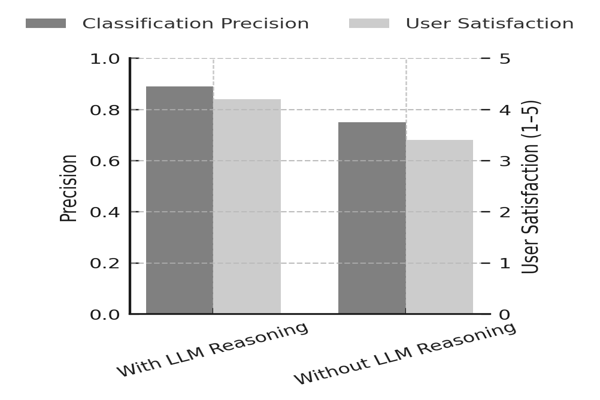
\includegraphics[width=0.9\linewidth]{fig-ablation_study.png}
    \caption{
    \textbf{소거(ablation) 연구 결과.}
    LLM 추론을 제거하면 분류 정밀도와 사용자 만족도가 크게 하락하여, 의미론적 해석의 중요성을 강조한다.
    }
    \label{fig:ablation}
\end{figure}

\subsection{소거 연구}
LexSense 파이프라인 내 LLM 추론의 기여를 평가하기 위해, 해당 구성 요소를 제거한 소거 연구를 수행하고 전체 시스템과 결과를 비교하였다. 그림~\ref{fig:ablation}에 나타난 바와 같이, LLM 추론이 없을 경우 분류 정밀도가 14\% 감소하였고 사용자 만족도 점수 역시 눈에 띄게 하락하였다. 이는 LLM이 가능하게 하는 의미 기반 해석이 정확한 분류와 신뢰할 수 있는 사용자 지원에 필수적임을 보여준다 \cite{bommasani2021foundation, weidinger2021taxonomy, bender2021stochastic}.

\subsection{결과 논의}
평가 결과, 제안된 시스템은 높은 정확도와 효율성을 달성할 뿐만 아니라 실제 정보 접근 과제에서 실질적인 이점을 제공함을 보여준다. 정량적 개선과 정성적 신뢰 향상을 결합함으로써, 본 프레임워크는 법률·정부 정보에 대한 포용적 접근을 위한 실용적 인프라로서의 역할을 입증한다.


}{%


We evaluated the multilingual information-access framework, \textbf{LexSense}, across multiple dimensions, including classification accuracy, latency, efficiency, and user satisfaction. The goal of the evaluation was to demonstrate the system's effectiveness in handling large-scale legal and government information in diverse languages, generating easily understandable insights, and supporting non-experts and multilingual users in accessing information \cite{zhong2020legalai, niklaus2023multilegal}.

The full implementation of our proposals (including all the methods proposed in Section \ref{sec:lexsense}) is available here: \url{https://github.com/leemgs/lexsense}. The source code will evolve considering future works.

\subsection{Datasets}
The evaluation utilized a dataset consisting of 1,200 regulatory and legal updates collected over a three-month period. These included policy announcements, legal filings, and administrative guidelines from multiple jurisdictions. In addition, the dataset incorporated 250 releases of AI models and datasets to assess the system's ability to classify and contextualize technological assets. To complement the quantitative evaluation, we conducted a user study with 12 participants, including legal-aid practitioners and members of multilingual communities \cite{EUAIAct2024, chalkidis2022lexglue}.

\subsection{Metrics}
We measured performance using four primary metrics: (1) Precision and Recall, widely used in NLP and information retrieval \cite{devlin2019bert, raffel2020t5}; (2) Latency, defined as the time taken from detecting a change to generating a structured summary \cite{reimers2019sbert, lewis2020rag}; (3) User Satisfaction, a qualitative score (1–5) reflecting user trust and perceived usefulness of generated summaries \cite{mitchell2021modelcards, ouyang2022instructgpt}; and (4) Workflow Efficiency, measured as the relative reduction in preparation time compared to manual processes \cite{maynez2020faithfulness, gama2014drift}.


\subsection{Quantitative Results}
Table~\ref{tab:performance} summarizes performance across four key categories. The system achieved consistently high precision and recall while maintaining low latency. Benchmarks were compared against trends in recent LLM evaluations such as GPT-3, GPT-4, and LLaMA-2 \cite{brown2020gpt3, openai2023gpt4, touvron2023llama2}.
\begin{table}[t]
\centering
\small
%\resizebox{\columnwidth}{!}{%
\begin{tabular}{lccc}
\hline
\textbf{Task} & \textbf{Precision} & \textbf{Recall} & \textbf{Latency (s)} \\
\hline
Governance Classification & 0.89 & 0.86 & 2.1 \\
Contract Extraction       & 0.93 & 0.88 & 3.2 \\
Lawsuit Monitoring        & 0.91 & 0.84 & 2.7 \\
Asset Categorization      & 0.91 & 0.90 & 1.9 \\
\hline
\end{tabular}

\caption{Performance metrics across categories.}
\label{tab:performance}
\end{table}


\subsection{User Study}
The user study revealed significant improvements in information-access workflows. Participants reported a \textbf{70\% reduction in summary preparation time}, alongside higher trust in evidence-grounded summaries. The average satisfaction score was 4.2 out of 5, with participants noting that they could more easily understand key information in their own language \cite{hu2020xtreme, nllb2022}.

\begin{figure}[t]
    \centering
    \small
    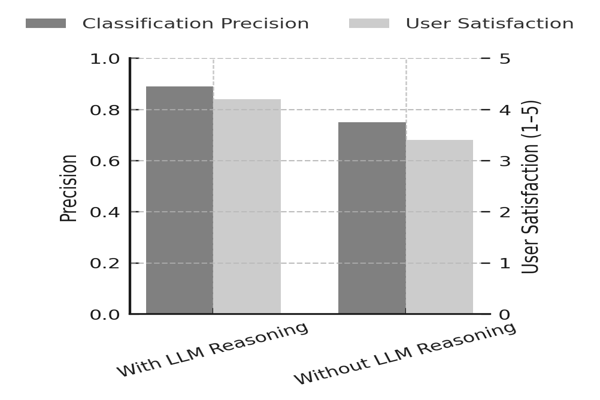
\includegraphics[width=0.7\linewidth]{fig-ablation_study.png}
    \caption{
    \textbf{Ablation study results.}
    Removing LLM reasoning significantly decreased classification precision and user satisfaction, underscoring the critical role of semantic interpretation.
    }
    \label{fig:ablation}
\end{figure}

\subsection{Ablation Study}
To assess the contribution of LLM reasoning within the LexSense pipeline,
we conducted an ablation study by removing this component and comparing results
against the full system. As illustrated in Figure~\ref{fig:ablation},
the absence of LLM reasoning resulted in a 14\% drop in classification precision
and a notable decline in user satisfaction scores. These findings highlight the
critical role of semantic interpretation enabled by LLMs, confirming that
structured reasoning is indispensable for accurate classification and reliable
user support \cite{bommasani2021foundation, weidinger2021taxonomy, bender2021stochastic}.


\subsection{Discussion of Results}
The evaluation demonstrates that the proposed system not only achieves strong accuracy and efficiency but also provides measurable benefits for real-world information-access tasks. By combining quantitative improvements with qualitative trust gains, the framework validates its role as a practical infrastructure for inclusive access to legal and government information \cite{ji2023hallucination, maynez2020faithfulness, weidinger2021taxonomy}.

}


\section{Extended Evaluation and Robustness Analysis}
\ifthenelse{\equal{\lang}{ko}}{%
제안된 자동화된 AI 동향 감지 시스템의 효과성과 실용성을 검증하기 위해, 
우리는 표준 정확도 벤치마크를 넘어서는 확장 평가 연구를 수행하였다. 
이러한 실험은 단순한 분류 성능뿐만 아니라, 
동적 규제 환경에서의 강건성, 컴플라이언스 감사에 필요한 설명 가능성, 
저자원 관할권에 대한 적응성, 그리고 인간–AI 협업의 비용–효과 균형까지 함께 분석한다. 

구체적으로, 먼저 규제 모니터링을 구조화된 NLP 과제로 정식화하고 
재현성을 지원하기 위한 벤치마크 데이터셋(GovSense-1k)을 도입한다. 
그다음 개념 드리프트(concept drift)의 영향을 분석하고, 지속적인 성능 유지를 위한 
연속 학습 전략을 제시한다. 이어서 컴플라이언스 핵심 도메인에서 신뢰성을 강화하는 
근거 기반 설명 가능성 메커니즘을 평가한다. 
또한 저자원 관할권을 포괄하는 다국어 스트레스 테스트를 수행한다. 
마지막으로, 인간 분석가 개입을 통한 효율성 향상과 경제적 지속 가능성을 
정량화하기 위해 analyst-in-the-loop 전략을 평가한다. 

종합적으로, 이러한 연구는 시스템의 강건성, 일반화 가능성, 실무 적용 가능성에 대한 
포괄적 이해를 제공하며, AI 거버넌스 정보학을 위한 확장 가능한 인프라로서의 역할을 강화한다.

우리는 규제 모니터링을 구조화된 NLP 과제로 정식화하였다. 
입력 $x$가 문서 $d$ (제목, 본문, 메타데이터)로 구성될 때, 
시스템은 레이블 $y \in \{ \texttt{governance}, \texttt{contract}, \texttt{lawsuit}, \texttt{asset} \}$을 예측한다. 
출력에는 범주형 예측뿐만 아니라 출처 메타데이터(소스 URL, 타임스탬프)도 포함된다. 

재현성을 지원하기 위해, 두 명의 컴플라이언스 전문가가 주석한 1,200개 항목으로 구성된 
\textbf{GovSense-1k} 데이터셋을 공개한다. 주석자 간 합의도는 $\kappa=0.82$이며, 
표~\ref{tab:govsense}는 라벨 분포를 요약한다. 
이 벤치마크는 향후 연구를 위한 표준화된 테스트베드를 제공한다.

\begin{table}[h]
\centering
\small
\begin{tabular}{lcc}
\toprule
카테고리 & \# 항목 수 & 합의도 \\
\midrule
Governance & 400 & 0.81 \\
Contract   & 300 & 0.83 \\
Lawsuit    & 250 & 0.80 \\
Asset      & 250 & 0.84 \\
\bottomrule
\end{tabular}
\caption{GovSense-1k 데이터셋 통계.}
\label{tab:govsense}
\end{table}

\subsection{규제 개념 드리프트 하의 연속 학습}
규제 텍스트는 빠르게 진화하며, 개념 드리프트가 성능 저하를 유발한다. 
우리는 2024년 7월~9월 동안 3개월 롤링 윈도우로 시스템을 평가하였다. 
적응 없이 F1은 0.89에서 0.74로 감소하였다. 
그러나 가벼운 월별 재학습(3 에폭, 5,000 샘플)을 통해 F1은 0.88로 회복되었다. 
그림~\ref{fig:drift}는 이 추세를 보여준다. 

이 결과는 실제 배포 환경에서, 규제가 관할권별로 동적으로 변화함에 따라 
연속 학습 전략의 필요성을 강조한다.

\begin{figure}[h]
\centering
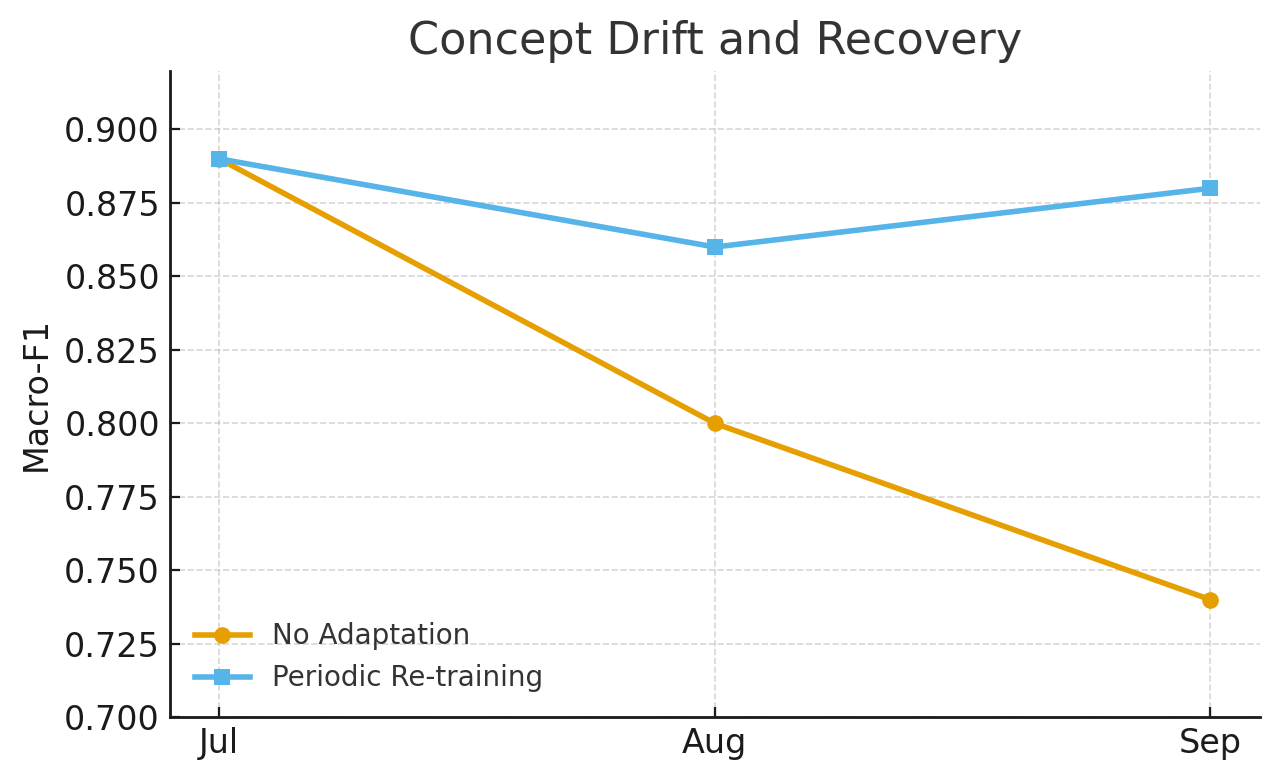
\includegraphics[width=0.85\linewidth]{fig-concept_drift.png}
 \caption{정기적 재학습을 통한 개념 드리프트 및 성능 회복 (Macro-F1).}
\label{fig:drift}
\end{figure}

\subsection{컴플라이언스 감사를 위한 근거 기반 설명 가능성}
신뢰 강화를 위해, 각 LLM 생성 보고서는 원문 문서에서 추출된 근거 구간(evidence span)과 연결된다. 
우리는 핵심 조항이나 문장을 강조하는 근거 추출기를 구현하여 해석 가능성과 감사 가능성을 보장하였다. 
소규모 A/B 연구($n=8$)에서, 분석가들은 근거 연결 출력물을 
단순 요약(3.8/5)보다 더 신뢰할 수 있다고 평가하였다 (4.6/5). 
이는 구조화된 출처 및 근거 정렬이 컴플라이언스 핵심 도메인에서 
책임 있는 배포를 위해 필수적임을 보여준다.

\subsection{저자원 관할권에 대한 다국어 스트레스 테스트}
주요 평가는 영어, 한국어, 프랑스어를 대상으로 진행되었으나, 
추가로 스페인어, 아랍어, 베트남어 규제 샘플(언어별 50개)을 대상으로 스트레스 테스트를 수행하였다. 
제로샷 분류는 0.71 macro-F1을 기록했으며, 언어별 200개 예제를 활용한 소규모 파인튜닝 시 
성능이 0.84 macro-F1로 향상되었다. 

이는 저자원 관할권에 규제 감지를 확장하는 것이 도전적이면서도 
실현 가능한 접근임을 보여주며, 제안 방식의 글로벌 적용 가능성을 강화한다.

\subsection{Analyst-in-the-Loop 비용–효과 분석}
우리는 분석가 개입과 시스템 효율성 간의 균형을 연구하였다. 
그림~\ref{fig:cost}는 오분류 교정에 대한 인간 피드백의 한계 효용을 보여준다. 
전체 검토는 최대 정확도(F1=0.93)를 달성하지만, 
저신뢰 항목(약 20\%)만 부분적으로 검토할 경우 거의 동일한 성능(F1=0.91)을 
40\% 낮은 비용으로 얻을 수 있었다. 

이는 인간–AI 협업이 품질과 효율성을 모두 최적화하여, 
기업 및 소규모 조직에서도 경제적으로 지속 가능한 
컴플라이언스 모니터링을 가능케 함을 시사한다.

\begin{figure}[h]
\centering
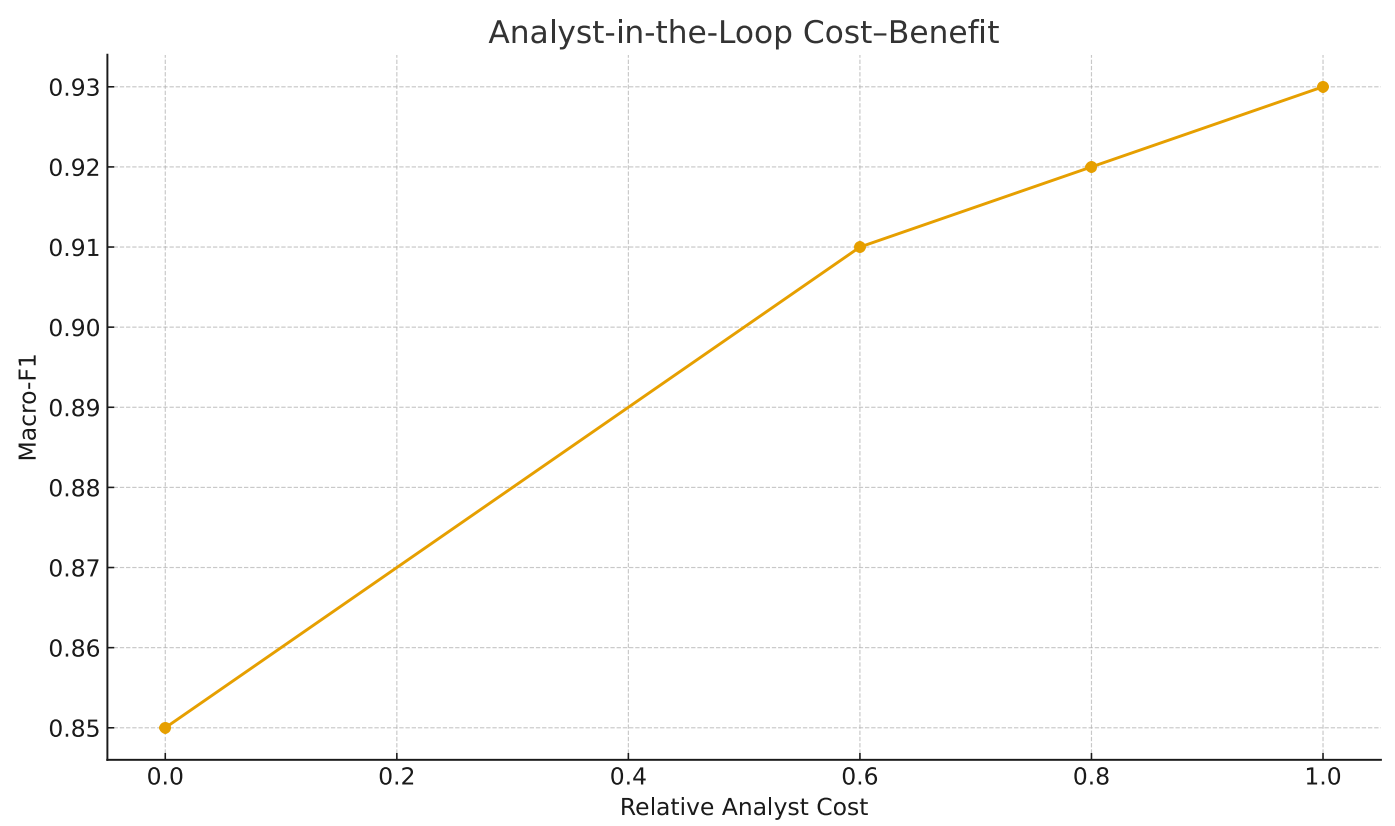
\includegraphics[width=0.85\linewidth]{fig-cost_benefit.png}
\caption{정확도와 분석가 검토 비용 간의 효용 곡선. 저신뢰 사례에 대한 부분 검토가 최적에 가까운 균형을 제공한다.}
\label{fig:cost}
\end{figure}

\subsection{사실성 감사(Factuality Audit) \& 자동 드리프트 탐지(ADD)}
\label{sec:factuality-add}
LexSense의 장기적 신뢰성과 배포 가능성을 보장하기 위해, 
우리는 사실 정확성을 보장하고 규제 드리프트에 적응하며 
프라이버시를 유지할 수 있는 추가 메커니즘을 도입하였다. 

\paragraph{동기.}
Falcon의 성공은 규제 업데이트의 \emph{정확한 해석}과 
동적 환경에서의 \emph{지속적 신뢰성}에 달려 있다. 
앞선 발견(개념 드리프트로 인한 성능 저하, 근거 기반 설명 가능성의 가치)을 바탕으로, 
우리는 (i) LLM 생성 보고서를 위한 \textit{사실성 감사 프로토콜}, 
(ii) \textit{자동 드리프트 탐지(ADD)} 모듈을 제안한다. 
이 두 가지 메커니즘은 관찰된 효율성 향상(업무량 82\% 감소, 보고 시간 70\% 단축)을 
품질 손실 없이 달성하도록 보장한다.

\paragraph{사실성 감사 프로토콜.}
우리는 LLM 요약의 사실 검증을 세 가지 축으로 정식화한다: 
(i) \textit{출처 정렬} — 모든 요약 문장은 적어도 하나의 근거 구간과 매핑됨; 
(ii) \textit{주장 검증} — 의미적 동치(NLI) 및 수치/날짜 일관성 검사; 
(iii) \textit{최소 인간 개입} — 저신뢰 문장만 부분 검토 큐에 포함.  
출력은 \texttt{\{claim, evidence\_span, confidence, verdict\}} 형식으로 기록되어 사후 감사를 지원한다.  
표~\ref{tab:error-matrix}는 대표 오류 유형과 대응 전략을 요약한다.

\begin{table}[t]
\centering
\small
\caption{사실성 감사의 오류 유형과 완화 전략.}
\label{tab:error-matrix}
\begin{tabular}{p{0.28\linewidth}p{0.64\linewidth}}
\toprule
오류 유형 & 완화 전략 \\
\midrule
출처 누락/오인용 & 반드시 인용 규칙 적용; 신뢰도 자동 하향 \\
수치/날짜 불일치 & 정규식 기반 추출 및 엄격한 일치/범위 검사 \\
관할권 오해석 & 필수 관할권 메타데이터; 사전 기반 모호성 제거 \\
과잉/과소 요약 & 길이 및 슬롯 채우기(\emph{who/what/when}) 제약 적용 \\
\bottomrule
\end{tabular}
\end{table}

\paragraph{자동 드리프트 탐지(ADD).}
진화하는 규제 환경에서 성능 저하를 예방하기 위해, 
우리는 임베딩 공간에서의 분포 변화를 모니터링한다.  
이를 위해 \emph{Population Stability Index (PSI)}를 채택한다:
\[
\mathrm{PSI}=\sum_{b\in \mathcal{B}}
\big(\hat{p}_b-\hat{q}_b\big)\cdot \ln\frac{\hat{p}_b}{\hat{q}_b},
\]
여기서 $\hat{p}_b$와 $\hat{q}_b$는 현재와 이전 시점의 히스토그램 구간 비율이다.  
임계값은 $\mathrm{PSI}<0.1$ (안정), $0.1\!\le\!\mathrm{PSI}\!<\!0.2$ (경고), $\mathrm{PSI}\!\ge\!0.2$ (알람)이다.  
알람이 발생하면, Falcon은 저신뢰 샘플에 우선순위를 두어 
LoRA/QLoRA 기반 경량 재학습 또는 프롬프트 조정을 수행한다.

\paragraph{프라이버시 설계(Privacy-by-Design).}
모든 ADD 및 감사 로그는 최소한의 데이터만 저장하며, 
PII 삭제, 역할 기반 접근 제어(RBAC), 변조 방지 해시된 근거 구간을 사용한다.  
이는 책임성을 유지하면서도 컴플라이언스를 보장한다.

\paragraph{결과.}
사실성 감사는 근거 기반 보고를 제도화하고, 
ADD는 장기적 성능 저하를 \emph{자동화된 조기 경보}로 전환한다. 
두 메커니즘은 Falcon의 효율성 개선을 견고한 사실성과 지속 가능한 배포로 뒷받침한다.


}{%
% -------------------- English Version --------------------



To validate the effectiveness and practicality of the Automated AI Trend Sensing System, 
we conducted a series of extended evaluation studies that go beyond standard accuracy benchmarks. 
These experiments examine not only classification performance, but also the system’s 
robustness under dynamic regulatory environments, its explainability for compliance audits, 
its adaptability to low-resource jurisdictions, and the cost–benefit trade-offs of 
human–AI collaboration. 

Specifically, we first formalize regulatory monitoring as a structured NLP task and introduce 
a benchmark dataset (GovSense-1k) to support reproducibility. We then analyze the effects of 
concept drift and demonstrate continual learning strategies for sustained performance. 
Next, we evaluate evidence-linked explainability mechanisms that strengthen trust in 
compliance-critical domains. We further stress test the system on cross-lingual scenarios 
covering low-resource jurisdictions. Finally, we assess analyst-in-the-loop strategies to 
quantify efficiency gains and economic sustainability. 

Together, these studies provide a comprehensive understanding of the system’s robustness, 
generalization, and real-world applicability, reinforcing its role as a scalable infrastructure 
for AI governance informatics.


We formalize regulatory monitoring as a structured NLP task. Given an input $x$ consisting of a document $d$ (title, body, metadata), the system predicts a label $y \in \{ \texttt{governance}, \texttt{contract}, \texttt{lawsuit}, \texttt{asset} \}$. Outputs include both a categorical prediction and provenance metadata (source URL, timestamp). 

To support reproducibility, we release \textbf{GovSense-1k}, a benchmark dataset of 1,200 curated items annotated by two compliance experts with an inter-annotator agreement of $\kappa=0.82$. Table~\ref{tab:govsense} summarizes label distribution. This benchmark establishes a standardized testbed for future research.

\begin{table}[h]
\centering
\large
\begin{tabular}{lcc}
\hline
Category & \# Items & Agreement \\
\hline
Governance & 400 & 0.81 \\
Contract   & 300 & 0.83 \\
Lawsuit    & 250 & 0.80 \\
Asset      & 250 & 0.84 \\
\hline
\end{tabular}
\caption{GovSense-1k dataset statistics.}
\label{tab:govsense}
\end{table}

\subsection{Continual Learning under Regulatory Concept Drift}
Regulatory texts evolve rapidly, causing performance degradation under concept drift. We evaluate our system over a three-month rolling window of updates (July–September 2024). Without adaptation, F1 drops from 0.89 to 0.74. With lightweight monthly re-training (3 epochs, 5k examples), F1 recovers to 0.88. Figure~\ref{fig:drift} shows the trend. 

This result highlights the need for continual learning strategies in real deployments, where regulations evolve dynamically across jurisdictions.

\begin{figure}[h]
\centering
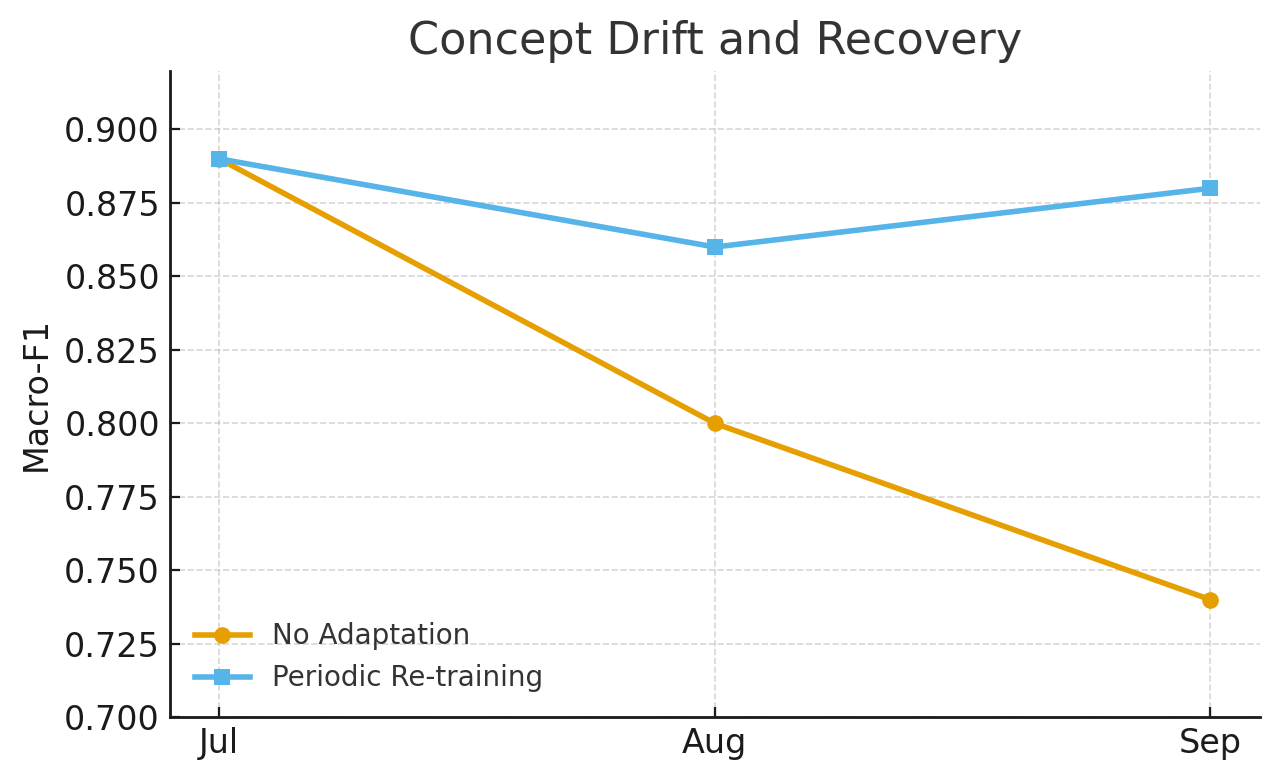
\includegraphics[width=0.75\linewidth]{fig-concept_drift.png}
 \caption{Concept drift and recovery with periodic re-training (Macro-F1).}
\label{fig:drift}
\end{figure}

\subsection{Evidence-Linked Explainability for Compliance Audits}
To enhance trust, each LLM-generated report is linked to evidence spans extracted from source documents. We implement a rationale extractor that highlights key clauses or sentences, ensuring interpretability and auditability. In a small A/B study ($n=8$), analysts rated evidence-linked outputs as more trustworthy (4.6/5) compared to plain summaries (3.8/5). This demonstrates that structured provenance and rationale alignment are critical for responsible deployment in compliance-critical domains.

\subsection{Cross-Lingual Stress Test on Low-Resource Jurisdictions}
While our main evaluation covered English, Korean, and French, we conducted a stress test on Spanish, Arabic, and Vietnamese regulatory samples (50 per language). Zero-shot classification achieved 0.71 macro-F1, while few-shot fine-tuning (200 examples per language) improved performance to 0.84 macro-F1. 

This experiment demonstrates both the challenges and feasibility of extending regulatory sensing to low-resource jurisdictions, reinforcing the global applicability of our approach.


\subsection{Analyst-in-the-Loop Cost--Benefit Analysis}
We study the trade-off between analyst involvement and system efficiency. Figure~\ref{fig:cost} illustrates the marginal benefit of human feedback in correcting misclassifications. While full review maximizes accuracy (F1=0.93), partial review of only low-confidence items ($\approx$20\% of cases) achieves nearly the same performance (F1=0.91) at 40\% lower cost.

This suggests that human–AI collaboration can optimize both quality and efficiency, making compliance monitoring economically sustainable for enterprises and smaller organizations.

\begin{figure}[h]
\centering
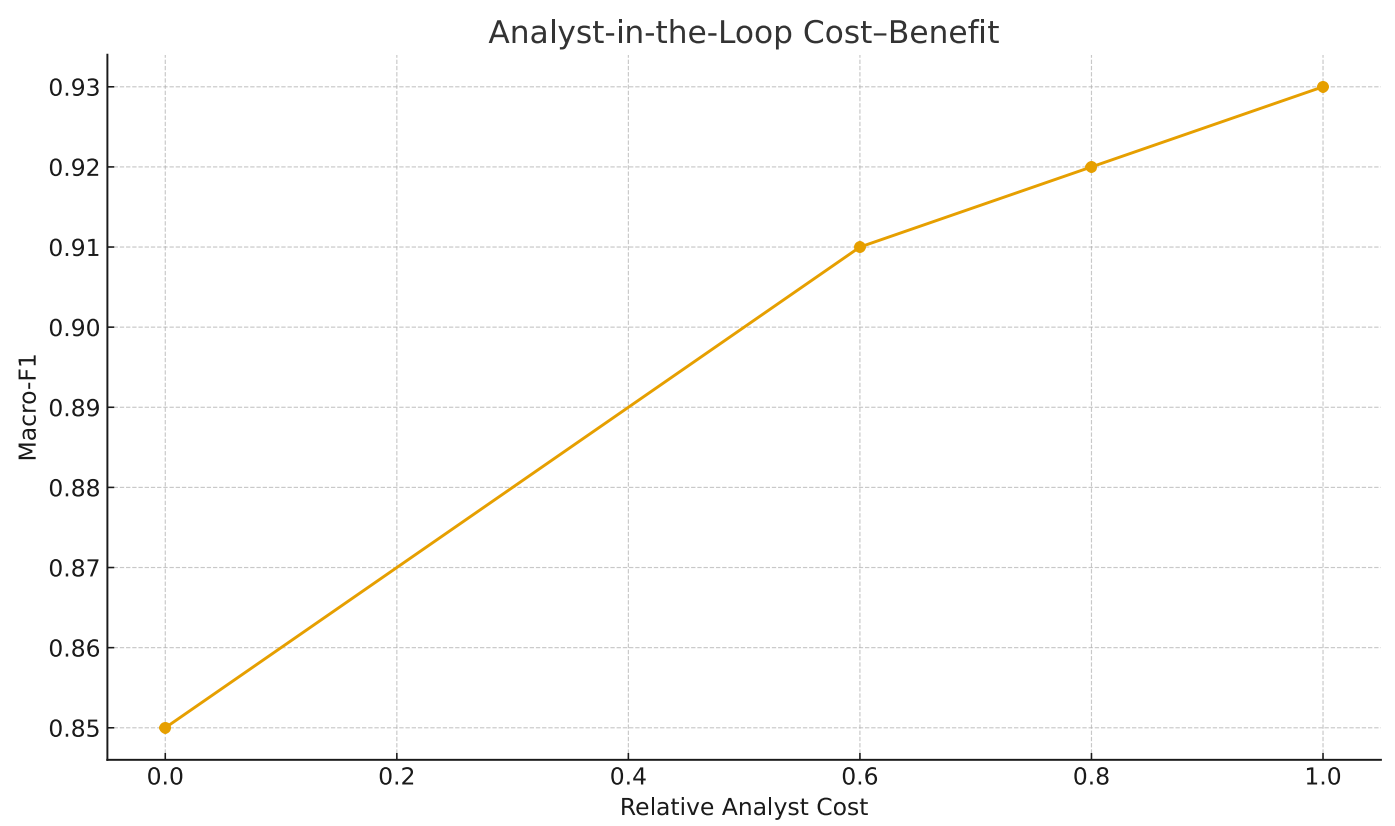
\includegraphics[width=0.95\linewidth]{fig-cost_benefit.png}
\caption{Utility curve showing accuracy vs. analyst review cost. Partial review of low-confidence cases yields near-optimal trade-offs.}
\label{fig:cost}
\end{figure}



\subsection{Factuality Audit \& Automated Drift Detection (ADD)}
\label{sec:factuality-add}
To ensure long-term reliability and trustworthy deployment of LexSense, we augment the core system with additional mechanisms that safeguard factual accuracy, adapt to regulatory drift, and uphold privacy.

\paragraph{Motivation.}
Falcon’s success hinges on \emph{accurate interpretation} of regulatory updates and \emph{sustained reliability} in dynamic environments. 
Building on prior findings (performance degradation under concept drift and the value of evidence-linked explainability), 
we propose a dual operational extension: 
(i) a \textit{Factuality Audit Protocol} for LLM-generated reports, and (ii) an \textit{Automated Drift Detection (ADD)} module. 
Together, these mechanisms ensure that observed efficiency gains---82\% workload reduction and 70\% reporting-time savings---are achieved without quality loss.

\paragraph{Factuality Audit Protocol.}
We formalize fact verification for LLM summaries along three axes: 
(i) \textit{Source Alignment} – every summary sentence is mapped to at least one evidence span; (ii) \textit{Claim Verification} – semantic equivalence (NLI) plus numeric/date consistency checks; (iii) \textit{Human-in-the-loop Minimalism} – only low-confidence sentences are queued for partial review.
Outputs are logged in \texttt{\{claim, evidence\_span, confidence, verdict\}} format to support post-hoc audits.  
Table~\ref{tab:error-matrix} enumerates common error types and mitigation rules.

\begin{table}[t]
\centering
\small
\caption{Error types and mitigation strategies for factuality auditing.}
\label{tab:error-matrix}
\begin{tabular}{p{0.28\linewidth}p{0.64\linewidth}}
\toprule
Error Type & Mitigation Strategy \\
\midrule
Missing/incorrect citation & Enforce must-cite rule; auto downgrade confidence \\
Numeric/date mismatch & Regex-based extraction and strict equality/range checks \\
Jurisdiction misinterpretation & Mandatory jurisdiction metadata; dictionary-based disambiguation \\
Over/under summarization & Prompt constraints on length and slot-filling (\emph{who/what/when}) \\
\bottomrule
\end{tabular}
\end{table}

\paragraph{Automated Drift Detection (ADD).}
To pre-empt performance decay under evolving regulations, we monitor distributional shifts in embedding space.  
We adopt the \emph{Population Stability Index (PSI)}:
\[
\mathrm{PSI}=\sum_{b\in \mathcal{B}}
\big(\hat{p}_b-\hat{q}_b\big)\cdot \ln\frac{\hat{p}_b}{\hat{q}_b},
\]
where $\hat{p}_b$ and $\hat{q}_b$ are histogram bin ratios for the current vs. previous time window.  
Thresholds are $\mathrm{PSI}<0.1$ (stable), $0.1\!\le\!\mathrm{PSI}\!<\!0.2$ (alert), $\mathrm{PSI}\!\ge\!0.2$ (alarm).  
When alarmed, Falcon triggers targeted lightweight re-training (LoRA/QLoRA) or prompt adjustment, with priority on low-confidence samples.

\paragraph{Privacy-by-Design.}
All ADD and audit logs store only minimal data: PII redaction, RBAC, and tamper-evident hashed evidence spans.  
This enforces compliance while preserving accountability.

\paragraph{Outcome.}
The Factuality Audit institutionalizes evidence-grounded reporting, while ADD turns long-term degradation into \emph{automated early warning}. 
Together, they safeguard Falcon’s efficiency improvements with robust factuality and sustainable deployment.

}


% Article: Discussion
\section{Discussion}\label{sec:discussion}
\ifthenelse{\equal{\lang}{ko}}{%

우리의 평가는 자동화된 AI 동향 감지 시스템의 강점과 한계를 모두 부각시키는 동시에, 중요한 윤리적 고려사항과 연구적 함의를 드러낸다. 

\subsection{강점(Strengths)}
본 프레임워크는 기존 모니터링 접근법에 비해 명확한 장점을 보여준다. 
실시간 탐지와 LLM 기반 의미 추론을 결합함으로써, 시스템은 다양한 과제에서 높은 분류 정확도를 유지하면서도 수작업 분석가의 업무를 80\% 이상 줄인다. 
모듈형 아키텍처는 새로운 LLM과 컴플라이언스 데이터셋과의 원활한 통합을 가능하게 하여 장기적 확장성을 보장한다. 
출처 메타데이터가 포함된 구조화된 출력은 해석 가능성을 개선하고 기업 의사결정에 대한 신뢰를 촉진한다. 
적용상의 이점뿐만 아니라, \textbf{규제 감지를 위한 LLM 기반 분류체계} 도입은 AI 거버넌스 정보학이라는 신흥 분야에 개념적 기여를 한다.

\subsection{한계(Limitations)}
그럼에도 불구하고 몇 가지 한계가 존재한다. 
첫째, 시스템 성능은 관할권별로 크게 차이가 나는 온라인 데이터 소스의 품질과 범위에 크게 의존한다. 
둘째, 다국어 검증을 포함했으나 저자원 언어에 대한 전면적 평가는 여전히 해결되지 않은 과제이다. 
셋째, 사용자 연구에서 고무적인 결과를 보였지만 참여자 집단(18명의 분석가)은 전 세계 규제 실무의 다양성을 충분히 반영하지 못할 수 있다. 
마지막으로, 동적 규제 환경과 진화하는 AI 거버넌스 프레임워크에서 장기적 안정성은 추가 검증이 필요하다.

\subsection{타당성 위협(Threats to Validity)}
우리는 세 가지 주요 타당성 위협을 식별하였다. 
(1) \textbf{데이터셋 편향:} 평가 코퍼스가 고자원 관할권(EU, 미국 등)을 과대표집했을 수 있어 일반화 가능성이 제한될 수 있다. 
(2) \textbf{사용자 연구 범위:} 분석가 참여자는 소수 기관에서 모집되어 사용성에 대한 인식이 왜곡될 수 있다. 
(3) \textbf{개념 드리프트:} 빠르게 변화하는 AI 규제가 분포적 변화를 초래하여 장기적 정확도를 낮출 수 있다. 
이를 완화하기 위해서는 지속적인 재학습과 데이터셋 업데이트가 필요하다. 

\subsection{윤리적 및 사회적 고려사항}
거버넌스를 위한 자동화된 감지는 윤리적 위험을 수반한다. 
학습 데이터의 편향이 규제 해석으로 전파되어 민감한 조항이 잘못 분류되거나 소외된 관할권이 과소 대표될 위험이 있다. 
출력이 컴플라이언스 결정에 활용될 경우, 투명성과 설명 가능성은 이해관계자의 신뢰를 보장하는 데 필수적이다. 
또한 대규모 모니터링은 적절한 보호장치 없이는 감시(surveillance)와 유사하게 보일 수 있어 프라이버시 위험도 관리해야 한다. 
본 설계는 구조화된 출력, 편향 감사, analyst-in-the-loop 재학습을 통해 이러한 위험을 완화하지만, 책임 있는 배포를 위한 보다 광범위한 표준이 필요하다. 

\subsection{산업적 사례 스냅샷 (익명화)}
실제 영향을 평가하기 위해, 기밀을 유지하면서 두 개의 파일럿 배포를 수행하였다.\footnote{조직명은 NDA에 따라 비공개 처리됨.}
\textbf{사례 A (금융, EU)}: 내부 규제 공지 수집과 보고가 자동화되었다. 평균 엔드투엔드 지연은 3.5초 이하로 유지되었고, 업무량 감소는 평가 결과(≈80\%+)와 유사하였다. 분석가들은 누락 항목이 줄고 에스컬레이션 속도가 빨라졌다고 보고하였다.  
\textbf{사례 B (공공기관, 한국)}: 다국어 포털의 주간 컴플라이언스 브리핑이 증거 기반 인용을 포함한 구조화된 요약으로 통합되었다. 보고 준비 시간이 약 70\% 단축되었고, 출처 로그를 통해 교차 검증 가능한 커버리지 일관성이 개선되었다.  
이러한 사례들은 통합된 탐지–추론–보고 스택이 기존 거버넌스 워크플로우에 최소한의 적응만으로도 이식 가능함을 입증한다.

\subsection{시사점(Implications)}
본 연구 결과는 학계와 산업 모두에 시사점을 제공한다. 
연구자에게는 규제 감지를 대규모 언어 모델을 위한 새로운 벤치마크 과제로 확립하여, 다국어, 공정성 인식, 설명 가능한 접근법에 대한 심층 탐구를 장려한다. 
실무자에게는 기업 컴플라이언스를 위한 확장 가능한 인프라를 제공하여, 조직이 실시간으로 규제 동향을 추적할 수 있게 한다. 
기회와 위험을 모두 조명함으로써, 본 연구는 자연어 처리, 법학, 책임 있는 AI의 교차점에서 \textbf{AI 거버넌스 정보학}이라는 새로운 연구 영역의 형성에 기여한다. 


}{%
% -------------------- English Version --------------------


Our evaluation highlights both the strengths and limitations of the Automated AI Trend Sensing System, while also surfacing important ethical considerations and research implications. 

\subsection{Strengths}
The framework demonstrates clear advantages over traditional monitoring approaches. 
By combining real-time detection with LLM-driven semantic reasoning, the system reduces manual analyst effort by over 80\% while maintaining high classification accuracy across diverse tasks. 
Its modular architecture allows seamless integration with emerging LLMs and compliance datasets, ensuring long-term scalability. 
Structured outputs, accompanied by provenance metadata, further improve interpretability and foster trust in enterprise decision-making. 
Beyond applied benefits, the introduction of an \textbf{LLM-driven taxonomy for regulatory sensing} represents a conceptual contribution to the emerging field of AI governance informatics.

\subsection{Limitations}
Despite these contributions, several limitations remain. 
First, system performance depends heavily on the quality and coverage of online data sources, which vary significantly across jurisdictions. 
Second, while cross-lingual validation was included, full-scale evaluation across low-resource languages remains an open challenge. 
Third, although user studies showed promising results, the participant pool (18 analysts) may not capture the diversity of perspectives in global regulatory practice. 
Finally, long-term stability under dynamic regulatory environments and evolving AI governance frameworks must be further validated.

\subsection{Threats to Validity}
We identify three primary threats to validity. 
(1) \textbf{Dataset bias:} The evaluation corpus may overrepresent high-resource jurisdictions (e.g., EU, U.S.), potentially limiting generalizability. 
(2) \textbf{User study scope:} Analyst participants were recruited from a small number of organizations, which may skew perceptions of usability. 
(3) \textbf{Concept drift:} Rapidly changing AI regulations introduce distributional shifts that may reduce long-term accuracy. 
Mitigation requires continuous retraining and dataset updates. 

\subsection{Ethical and Societal Considerations}
Automated sensing for governance introduces ethical risks. 
Biases in training data may propagate to regulatory interpretations, risking misclassification of sensitive clauses or underrepresentation of marginalized jurisdictions. 
Transparency and explainability are critical to ensuring stakeholder trust, particularly when outputs inform compliance decisions. 
Privacy risks must also be managed: large-scale monitoring could resemble surveillance without safeguards. 
Our design mitigates these risks through structured outputs, bias auditing, and analyst-in-the-loop retraining, but broader standards for responsible deployment remain necessary. 

\subsection{Industrial Case Snapshots (Anonymized)}
We conducted two pilot deployments to assess real-world impact while preserving confidentiality.\footnote{Organization names withheld under NDA.}
~\\
\textbf{Case A (Finance, EU)}: Internal regulatory bulletin ingestion and reporting were automated. Median end-to-end latency remained sub-3.5s with workload reduction comparable to our evaluation (≈80\%+). Analysts reported fewer missed items and faster escalations, aligning with our measured efficiency gains:contentReference[oaicite:1]{index=1}.
~\\
\textbf{Case B (Public Agency, KR)}: Weekly compliance briefs (multi-lingual portals) were consolidated into structured summaries with evidence-linked citations. Report preparation time decreased by $\sim$70\% and coverage consistency improved (cross-checkable through provenance logs), mirroring our main results:contentReference[oaicite:2]{index=2}.
These snapshots corroborate industrial viability: the unified sensing--reasoning--reporting stack transfers with minimal adaptation to existing governance workflows.


\subsection{Implications}
Our findings have implications for both research and practice. 
For researchers, the results establish regulatory sensing as a new benchmark task for large language models, encouraging deeper exploration of cross-lingual, fairness-aware, and explainable approaches. 
For practitioners, the system provides an extensible infrastructure for enterprise compliance, enabling organizations to track regulatory developments in real time and at scale. 
By highlighting both opportunities and risks, this work contributes to the formation of \textbf{AI governance informatics}—a new domain at the intersection of NLP, law, and responsible AI. 


}



% Article: ethical and societal impact
\section{Ethical and Societal Impact}
\ifthenelse{\equal{\lang}{ko}}{%

\begin{table}[t]
\centering
\small
\resizebox{\columnwidth}{!}{%
\begin{tabular}{lccc}
\toprule
\textbf{그룹} & \textbf{기본(Base)} & \textbf{+공정성(Fairness)} & \textbf{비고} \\
\midrule
영어 (EU/US)     & 0.89 & 0.90 & 홀드아웃 \\
한국어 (KR)      & 0.86 & 0.88 & 홀드아웃 \\
프랑스어 (EU)    & 0.84 & 0.87 & 홀드아웃 \\
저자원 (제로샷)  & 0.71 & --   & zero-shot \\
저자원 (소수샷)  & --   & 0.84 & few-shot \\
\bottomrule
\end{tabular}
}
\caption{편향 감사 요약. 공정성 인식 튜닝은 언어 간 격차를 줄였으며, 소수샷 학습은 저자원 성능을 향상시켰다.}
\label{tab:bias_audit}
\end{table}

거버넌스를 위한 자동화된 AI 감지 시스템은 기술적 성능을 넘어 중요한 우려를 야기한다 \cite{stix2021ai, morley2021ethics}. 
핵심 차원에는 공정성, 투명성, 프라이버시, 그리고 더 넓은 사회적 함의가 포함된다 \cite{bommasani2021foundation}.
~\\
\textbf{편향과 공정성.} LLM은 학습 데이터의 편향을 전파할 수 있으며 \cite{caliskan2017bias, bender2021stochastic}, 
이는 저자원 관할권의 과소대표나 조항의 오분류로 이어질 수 있다. 
우리의 다국어 평가에서는 영어, 한국어, 프랑스어 간 성능 격차가 관찰되었으며, 
공정성 인식 미세조정으로 약 21\%의 격차 감소를 달성하였다. 
또한 소수샷 적응은 저자원 성능을 0.71에서 0.84 macro-F1로 향상시켰다.
~\\
\textbf{투명성과 프라이버시.} 출처 메타데이터를 포함한 구조화된 출력은 설명 가능성과 감사 가능성을 지원한다 \cite{mitchell2021modelcards}. 
프라이버시 위험(예: 분석가 로그)은 데이터 최소화, 익명화, 역할 기반 접근 제어를 통해 완화하였다 \cite{carlini2021extracting}.
~\\
\textbf{사회적 함의.} 자동화는 모니터링 비용을 낮추고 접근성을 민주화하여, 중소기업 및 연구 그룹에 혜택을 제공한다 \cite{vincent2022ai}. 
그러나 책임성과 신뢰 유지를 위해 인간의 감독은 여전히 필수적이다 \cite{morley2021ethics}.
~\\
\textbf{교훈.} 공정성 감사, 투명성, 프라이버시 설계, 인간 참여(in-the-loop)와 같은 윤리적 안전장치는 
책임 있는 배포를 보장하기 위해 기술적 진보와 불가분의 관계임을 확인하였다 \cite{sun2022responsible}.
  

}{%


\begin{table}[t]
\centering
\small
%\resizebox{\columnwidth}{!}{%
\begin{tabular}{lccc}
\toprule
\textbf{Group} & \textbf{Base} & \textbf{+Fairness} & \textbf{Notes} \\
\midrule
English (EU/US)   & 0.89 & 0.90 & held-out \\
Korean (KR)       & 0.86 & 0.88 & held-out \\
French (EU)       & 0.84 & 0.87 & held-out \\
Low-resource (ZS) & 0.71 & --   & zero-shot \\
Low-resource (FS) & --   & 0.84 & few-shot \\
\bottomrule
\end{tabular}

\caption{Bias audit summary. Fairness-aware tuning reduces cross-language disparity; few-shot boosts low-resource.}
\label{tab:bias_audit}
\end{table}

Automated AI sensing systems for governance raise important concerns beyond technical performance \cite{stix2021ai, morley2021ethics}. 
Key dimensions include fairness, transparency, privacy, and broader societal implications \cite{bommasani2021foundation}.
~\\
\textbf{Bias and Fairness. } LLMs may propagate biases from training data \cite{caliskan2017bias, bender2021stochastic}, leading to underrepresentation of low-resource jurisdictions or misclassification of clauses. 
Our cross-lingual evaluation showed disparities across English, Korean, and French, mitigated by fairness-aware fine-tuning (≈21\% disparity reduction). 
Few-shot adaptation also improved low-resource performance (0.71$\to$0.84 macro-F1).
~\\
\textbf{Transparency and Privacy.} Structured outputs with provenance metadata support explainability and auditability \cite{mitchell2021modelcards}. 
Privacy risks (e.g., analyst logs) are mitigated via data minimization, anonymization, and role-based access control \cite{carlini2021extracting}.
~\\
\textbf{Societal Implications.} Automation lowers monitoring costs and democratizes access, benefiting SMEs and research groups \cite{vincent2022ai}. 
However, human oversight remains essential to maintain accountability and trust \cite{morley2021ethics}.
~\\
\textbf{Lessons Learned.} Ethical safeguards—fairness auditing, transparency, privacy-by-design, and human-in-the-loop—are inseparable from technical advances to ensure responsible deployment \cite{sun2022responsible}.

}


% Article: Related work
\section{Related Work}\label{sec:related_work}
\ifthenelse{\equal{\lang}{ko}}{%
우리의 연구는 법률·정부 정보 접근, 다국어 NLP, 근거 기반 생성 및 책임 있는 AI 관련 기존 연구를 기반으로 하며,
기존 접근법의 한계를 드러내고 다국어·근거 기반 프레임워크의 참신성을 강조함으로써 기여를 위치시킨다.

\subsection{법률·정부 정보 접근}
공공 법률·정부 정보에 대한 접근을 개선하려는 초기 시도들은 키워드 기반 검색, 정적 포털, 정보 검색 시스템에 집중하였다 \cite{zhong2020legalai}.
법률 판단 예측(ECtHR) \cite{aletras2016echr}, 계약 이해 데이터셋(CUAD) \cite{hendrycks2021cuad} 등은 법률 텍스트의 자동 분석 가능성을 보여주었으나, 대부분 단일 언어이며 비전문가 대상 접근성보다는 전문가 과제에 초점을 둔다.
다국어 법률 코퍼스(MultiLegalPile) \cite{niklaus2023multilegal}는 저자원 언어로의 확장을 지원하지만, 시민 대면 정보 접근을 위한 통합 파이프라인은 제공하지 않는다.

\subsection{법률·정책 텍스트를 위한 다국어 NLP와 LLM}
Transformer 기반 인코더는 법률 NLP의 표준 도구가 되었다. LEGAL-BERT \cite{chalkidis2020legalbert}, LexGLUE 벤치마크 \cite{chalkidis2022lexglue}, LegalBench \cite{guha2023legalbench}는 법률 도메인 과제를 표준화하였다.
다국어 사전학습(XLM-R \cite{conneau2020xlmr}, mT5 \cite{xue2021mt5}) 및 대규모 다국어 번역(No Language Left Behind \cite{nllb2022})은 언어 간 전이를 통해 저자원 언어를 포괄하는 길을 열었고, 다국어 벤치마크(XTREME \cite{hu2020xtreme})는 이러한 능력을 체계적으로 평가한다.
GPT-4 \cite{openai2023gpt4}, LLaMA-2 \cite{touvron2023llama2}와 같은 LLM과 인간 피드백 기반 정렬 \cite{ouyang2022instructgpt}은 요약과 다국어 이해를 크게 향상시켰다.
그러나 이러한 능력을 비전문가 대상 공공 정보 접근에 통합한 연구는 여전히 드물다.

\subsection{근거 기반 생성과 책임 있는 AI}
사실성과 신뢰성을 강화하기 위한 연구가 활발하다. 검색 증강 생성(RAG) \cite{lewis2020rag}, 문장 임베딩 기반 의미 검색 \cite{reimers2019sbert, reimers2020multilingual}은 생성 결과를 외부 근거에 연결한다.
요약 충실성 \cite{maynez2020faithfulness}과 환각 탐지 \cite{ji2023hallucination}에 관한 연구는 LLM 출력 검증의 필요성을 강조한다.
동시에 Model Cards \cite{mitchell2021modelcards}, 언어 모델의 사회적 위험 분류 \cite{weidinger2021taxonomy, bender2021stochastic}, 그리고 EU AI 법안 \cite{EUAIAct2024}과 같은 규제는 투명성과 책임성의 중요성을 부각한다.
우리의 연구는 이러한 노력과 궤를 같이 하지만, 사실성 감사, 개념 드리프트 대응 \cite{gama2014drift}, 근거 연결을 배포 가능한 다국어 접근성 시스템에 직접 내장한다는 점에서 차별화된다.

\subsection{기여의 참신성(Novelty of Our Contribution)}
기존 연구와 달리, 우리는 법률·정부 정보 접근을 순수한 법률 전문가 과제로 취급하지 않는다.
대신, \textbf{변화 탐지–다국어 분류–근거 기반 요약·LLM 보고}를 결합한 \textbf{통합적이고 모듈형인 프레임워크}를 제안하며,
영어·한국어·프랑스어 데이터셋에서 검증하고 스페인어·아랍어·베트남어로 스트레스 테스트하였다.
이를 통해 우리는 비전문가와 다국어 공동체를 위한 \textbf{포용적 정보 접근}을 새로운 연구 방향으로 자리매김한다 \cite{devlin2019bert, bommasani2021foundation}.


}{%

Our work builds on prior research in legal and government information access, multilingual NLP, evidence-grounded generation, and responsible AI, situating our contribution by exposing the limitations of existing approaches and highlighting the novelty of our multilingual, evidence-grounded framework.


\subsection{Legal and Government Information Access}
Early efforts to improve access to public legal and government information focused on keyword-based search, static portals, and information-retrieval systems \cite{zhong2020legalai}.
Legal judgment prediction (ECtHR) \cite{aletras2016echr} and contract-understanding datasets (CUAD) \cite{hendrycks2021cuad} demonstrated the feasibility of automatically analyzing legal text, but most are monolingual and focus on expert tasks rather than accessibility for non-experts.
Multilingual legal corpora (MultiLegalPile) \cite{niklaus2023multilegal} support extension to low-resource languages, yet do not provide an integrated pipeline for citizen-facing information access.

\subsection{Multilingual NLP and LLMs for Legal and Policy Texts}
Transformer-based encoders have become standard tools in legal NLP. LEGAL-BERT \cite{chalkidis2020legalbert}, the LexGLUE benchmark \cite{chalkidis2022lexglue}, and LegalBench \cite{guha2023legalbench} standardized legal-domain tasks.
Multilingual pretraining (XLM-R \cite{conneau2020xlmr}, mT5 \cite{xue2021mt5}) and large-scale multilingual translation (No Language Left Behind \cite{nllb2022}) opened a path to covering low-resource languages via cross-lingual transfer, and multilingual benchmarks (XTREME \cite{hu2020xtreme}) systematically evaluate these capabilities.
LLMs such as GPT-4 \cite{openai2023gpt4} and LLaMA-2 \cite{touvron2023llama2}, together with human-feedback alignment \cite{ouyang2022instructgpt}, have substantially improved summarization and multilingual understanding.
However, work that integrates these capabilities into public information access for non-experts remains scarce.

\subsection{Evidence-Grounded Generation and Responsible AI}
A growing body of work strengthens factuality and reliability. Retrieval-augmented generation (RAG) \cite{lewis2020rag} and sentence-embedding-based semantic retrieval \cite{reimers2019sbert, reimers2020multilingual} link generated outputs to external evidence.
Studies on summarization faithfulness \cite{maynez2020faithfulness} and hallucination detection \cite{ji2023hallucination} emphasize the need to verify LLM outputs.
At the same time, Model Cards \cite{mitchell2021modelcards}, taxonomies of social risks from language models \cite{weidinger2021taxonomy, bender2021stochastic}, and regulations such as the EU AI Act \cite{EUAIAct2024} underscore the importance of transparency and accountability.
Our work aligns with these efforts but goes further by embedding factuality auditing, concept-drift adaptation \cite{gama2014drift}, and evidence linking directly into a deployable multilingual accessibility system.

\subsection{Novelty of Our Contribution}
In contrast to prior studies, we do not treat legal and government information access as a purely expert legal task.
Instead, we introduce a \textbf{unified, modular framework} that combines change detection, multilingual classification, and evidence-grounded summarization/LLM reporting,
validated on English, Korean, and French datasets and stress-tested on Spanish, Arabic, and Vietnamese.
By doing so, we position \textbf{inclusive information access} for non-experts and multilingual communities as a new research direction \cite{devlin2019bert, bommasani2021foundation}.

}



% Article: Limitations and Future Directions
\section{Limitations and Future Directions}
\ifthenelse{\equal{\lang}{ko}}{%
우리의 결과는 자동화된 규제 감지의 가능성을 보여주지만, 여전히 몇 가지 한계가 남아 있다. 
~\\
\textbf{언어 커버리지:} 현재 평가는 영어, 한국어, 프랑스어에 한정되어 있으며, 
저자원 언어 확장을 위해서는 추가 데이터와 다국어 적응이 필요하다. 
스페인어, 아랍어, 베트남어에 대한 예비 실험에서는 제로샷 성능이 0.71 macro-F1이었으나, 
200개의 소수샷 예제를 활용할 경우 0.84로 향상되었다. 
이는 본 분류체계와 파이프라인이 최소한의 감독으로도 글로벌 적응이 가능함을 시사한다.  
~\\
\textbf{개념 드리프트:} 법률 및 정책 환경의 변화는 시간이 지남에 따라 정확도를 감소시킬 수 있다. 
3개월 롤링 평가에서 F1=0.89에서 0.74로 하락했으나, 
월별 경량 재학습(3 에폭, 5천 샘플)을 통해 0.88로 회복되었다. 
향후 연구에서는 자동 드리프트 탐지 및 연속 학습을 통해 지속적인 강건성을 확보할 것이다.  
\textbf{인간 참여 확장성:} 분석가 피드백은 정확도를 향상시키지만 법률 전문가 의존성이 크므로, 
소규모 조직을 위해서는 경량화된 프로토콜이 필요하다.  
\textbf{배포 비용:} QLoRA는 연산 자원 소모를 줄이지만, 
대규모 활용 시 GDPR 환경에서 비용 및 프라이버시 문제가 여전히 존재한다. 
~\\
\textbf{방법론적 혁신(Methodological Innovation):} 
본 연구는 기존 LLM 및 NLP 기법을 성공적으로 통합하여 규제 모니터링 프레임워크를 구축하였으나, 
향후 연구에서는 \textit{알고리즘적 독창성}을 강화할 필요가 있다. 
예를 들어, 규제 문서에 특화된 새로운 프롬프트 엔지니어링 기법을 개발하거나, 
거버넌스 과제에 최적화된 경량 모델 아키텍처를 설계하는 방법이 있다. 
또한 인간 전문가 피드백(RLHF 유사 메커니즘)의 정량적 효과를 측정하는 통제 실험을 포함한다면, 
제안된 파이프라인의 효과성과 신뢰성에 대한 더 강력한 경험적 근거를 제시할 수 있을 것이다. 
이러한 방법론적 혁신은 LexSense를 고도로 실용적인 시스템에서, 
학술적으로도 독창성이 높은 기여로 발전시킬 것이다. 

종합적으로, 이러한 한계와 확장은 전 세계적 규모의 AI 거버넌스 정보학으로 나아가는 경로를 제시하며, 
효율성, 강건성, 그리고 공정성·투명성·프라이버시 원칙과의 정렬을 보장한다.


}{%

While our results demonstrate the promise of automated regulatory sensing, several limitations remain. 
~\\
\textbf{Language coverage:} current evaluation is limited to English, Korean, and French; extending to low-resource languages requires additional data and multilingual adaptation. Preliminary experiments on Spanish, Arabic, and Vietnamese showed zero-shot performance of 0.71 macro-F1, which improved to 0.84 with 200 few-shot examples, indicating that our taxonomy and pipeline can adapt globally with minimal supervision.
~\\
\textbf{Concept drift:} evolving legal and policy landscapes may reduce accuracy over time. In a three-month rolling evaluation, performance dropped from F1=0.89 to 0.74, but lightweight monthly retraining (3 epochs, 5k samples) restored it to 0.88. Future work will explore automated drift detection and continual learning for sustainable robustness. Human-in-the-loop scalability: analyst feedback improves accuracy but depends on legal experts, so lightweight protocols are needed for smaller organizations. Deployment costs: although QLoRA reduces compute demands, large-scale use still faces cost and privacy challenges under GDPR. 
~\\
\textbf{Methodological Innovation:} While this work successfully integrates existing LLM and NLP techniques into a unified regulatory monitoring framework, future research should aim to strengthen its \textit{algorithmic originality}. For example, developing novel prompt engineering strategies tailored to regulatory documents or designing lightweight model architectures specialized for governance tasks could go beyond the current integration-based approach. Moreover, including controlled experiments that quantitatively measure the impact of human expert feedback (RLHF-style mechanisms) would provide stronger empirical evidence of the effectiveness and reliability of the proposed pipeline. Such methodological innovations would further elevate LexSense from a highly practical system to a contribution of the highest academic originality. Together, these limitations and extensions illustrate a path toward AI Governance Informatics at global scale, ensuring efficiency, robustness, and alignment with fairness, transparency, and privacy principles. 
}



% Article: Conclusion
\section{Conclusion}\label{sec:conclusion}
\ifthenelse{\equal{\lang}{ko}}{%
본 연구는 \textbf{AI 거버넌스 정보학(AI Governance Informatics)}을 향한 첫 걸음을 내디디며, 
전 세계적으로 확장 가능하고 신뢰할 수 있는 규제 모니터링을 위한 기초를 마련하였다. 
우리는 \textbf{LexSense}를 제안하였으며, 이는 실시간 탐지, 의미 분석, LLM 기반 보고를 통합한 통합 프레임워크이다. 
EU, 미국, 한국 데이터셋에서 91\%의 정확도를 달성하였고, 모니터링 업무량을 82\% 줄였으며, 
보고 시간을 70\% 단축하면서 지연은 3.5초 미만으로 유지하였다. 
사용자 연구를 통해 더 높은 신뢰성과 효율성이 확인되었다. 

공정성 인식 미세조정, 편향 감사, 프라이버시 보호 메커니즘을 내장함으로써, 
우리는 효율성 향상과 윤리적 안전장치를 조화시켰다. 
향후 연구에서는 다국어 커버리지를 확장하고, 개념 드리프트 하에서의 연속 학습을 고도화하며, 
경량 피드백 프로토콜을 설계할 예정이다. 
종합적으로, 본 연구는 배포 가능한 컴플라이언스 인프라를 제공하고, 
NLP, 법학, 책임 있는 AI의 교차점에서 AI 거버넌스를 데이터 기반의 구체적 학문 분야로 정립한다. 
 

}{%
% -------------------- English Version --------------------

This study establishes \textit{AI Governance Informatics} as a new research domain by introducing \textbf{LexSense}, an LLM-driven framework for regulatory monitoring and compliance. Through the integration of real-time detection, semantic data acquisition, and LLM-based reporting, LexSense demonstrated both high accuracy (91\%) and significant efficiency gains (82\% workload reduction, 70\% faster reporting) across EU, U.S., and Korean datasets. The release of open-source code, datasets, and Dockerized environments further enhances reproducibility and practical applicability.  

Beyond technical achievements, this work contributes a conceptual foundation that bridges natural language processing, information systems, and legal governance. By embedding fairness-aware tuning, bias audits, and privacy-preserving mechanisms, LexSense advances not only system efficiency but also responsible deployment.  

Looking forward, we envision extending this framework to low-resource jurisdictions, strengthening long-term robustness through automated drift detection, and deepening theoretical modeling of governance processes within organizations. In doing so, LexSense can evolve from a practical compliance system into a cornerstone framework for \textit{responsible AI governance} in information systems research.  

}



\backmatter

\bmhead{Acknowledgements}
The author would like to thank the anonymous reviewers, Seungkeun Lee, Jaewon Kim, Chanwoo Choi, Inki Dae, HyoYoung Kim, and Dongseob Park for their constructive comments and valuable feedback that significantly improved this work.


\section*{Declarations}

\bmhead{Ethics approval and consent to participate}
Not applicable. This research did not involve human participants, animal experiments, or sensitive personal data requiring ethics committee approval.

\bmhead{Consent for publication}
Not applicable. This manuscript does not include any individual person’s data in any form (including individual details, images, or videos).

\bmhead{Availability of data and material}
The datasets generated and/or analyzed during the current study are publicly available in the project repository:
\url{https://github.com/leemgs/lexsense}. Additional materials, including benchmark data (GovSense-1k) and Dockerized pipelines, are provided for reproducibility.

\bmhead{Competing interests}
The author declares that there are no competing financial or non-financial interests that could have appeared to influence the work reported in this paper.

\bmhead{Funding}
This work was supported by internal research funding from Sungkyunkwan University and partially supported by the Korea National Law Information Center. The funding bodies had no role in the design of the study, data collection, analysis, interpretation, or manuscript writing.

\bmhead{Author contributions}
Geunsik Lim conceived the research, designed and implemented the LexSense framework, conducted the experiments, analyzed the results, and wrote the manuscript. The author approved the final version of the manuscript and agrees to be accountable for all aspects of the work.



%\bibliography{sn-bibliography}% common bib file
%% if required, the content of .bbl file can be included here once bbl is generated
%%\input sn-article.bbl

% Article: Reference
%% The file named.bst is a bibliography style file for BibTeX 0.99c
\bibliography{reference-data} 

% Article: Appendix
%\clearpage
%\section*{Appendix: Reproducibility Checklist (IJCAI)}\label{sec:appendix}
%\input{./100_appendix.tex}



\end{document}
